% Options for packages loaded elsewhere
\PassOptionsToPackage{unicode}{hyperref}
\PassOptionsToPackage{hyphens}{url}
%
\documentclass[
]{article}
\usepackage{amsmath,amssymb}
\usepackage{iftex}
\ifPDFTeX
  \usepackage[T1]{fontenc}
  \usepackage[utf8]{inputenc}
  \usepackage{textcomp} % provide euro and other symbols
\else % if luatex or xetex
  \usepackage{unicode-math} % this also loads fontspec
  \defaultfontfeatures{Scale=MatchLowercase}
  \defaultfontfeatures[\rmfamily]{Ligatures=TeX,Scale=1}
\fi
\usepackage{lmodern}
\ifPDFTeX\else
  % xetex/luatex font selection
\fi
% Use upquote if available, for straight quotes in verbatim environments
\IfFileExists{upquote.sty}{\usepackage{upquote}}{}
\IfFileExists{microtype.sty}{% use microtype if available
  \usepackage[]{microtype}
  \UseMicrotypeSet[protrusion]{basicmath} % disable protrusion for tt fonts
}{}
\makeatletter
\@ifundefined{KOMAClassName}{% if non-KOMA class
  \IfFileExists{parskip.sty}{%
    \usepackage{parskip}
  }{% else
    \setlength{\parindent}{0pt}
    \setlength{\parskip}{6pt plus 2pt minus 1pt}}
}{% if KOMA class
  \KOMAoptions{parskip=half}}
\makeatother
\usepackage{xcolor}
\usepackage[margin=1in]{geometry}
\usepackage{longtable,booktabs,array}
\usepackage{calc} % for calculating minipage widths
% Correct order of tables after \paragraph or \subparagraph
\usepackage{etoolbox}
\makeatletter
\patchcmd\longtable{\par}{\if@noskipsec\mbox{}\fi\par}{}{}
\makeatother
% Allow footnotes in longtable head/foot
\IfFileExists{footnotehyper.sty}{\usepackage{footnotehyper}}{\usepackage{footnote}}
\makesavenoteenv{longtable}
\usepackage{graphicx}
\makeatletter
\def\maxwidth{\ifdim\Gin@nat@width>\linewidth\linewidth\else\Gin@nat@width\fi}
\def\maxheight{\ifdim\Gin@nat@height>\textheight\textheight\else\Gin@nat@height\fi}
\makeatother
% Scale images if necessary, so that they will not overflow the page
% margins by default, and it is still possible to overwrite the defaults
% using explicit options in \includegraphics[width, height, ...]{}
\setkeys{Gin}{width=\maxwidth,height=\maxheight,keepaspectratio}
% Set default figure placement to htbp
\makeatletter
\def\fps@figure{htbp}
\makeatother
\setlength{\emergencystretch}{3em} % prevent overfull lines
\providecommand{\tightlist}{%
  \setlength{\itemsep}{0pt}\setlength{\parskip}{0pt}}
\setcounter{secnumdepth}{-\maxdimen} % remove section numbering
\ifLuaTeX
  \usepackage{selnolig}  % disable illegal ligatures
\fi
\IfFileExists{bookmark.sty}{\usepackage{bookmark}}{\usepackage{hyperref}}
\IfFileExists{xurl.sty}{\usepackage{xurl}}{} % add URL line breaks if available
\urlstyle{same}
\hypersetup{
  pdftitle={Documentation -- wetlandP\_v2.1},
  pdfauthor={Adrian Wiegman},
  hidelinks,
  pdfcreator={LaTeX via pandoc}}

\title{Documentation -- wetlandP\_v2.1}
\author{Adrian Wiegman}
\date{01 November, 2023}

\begin{document}
\maketitle

{
\setcounter{tocdepth}{2}
\tableofcontents
}
\hypertarget{about}{%
\subsection{About}\label{about}}

The wetlandP\_v2.1 model is an ordinary differential equation model
developed for estimating phosphorus (P) retention in riparian wetlands
with a range of soil and hydrologic conditions. The model is forced by
daily hydroclimatic inputs and is designed to simulate dynamics of soil,
water, and vegetation on time scales that range from weeks (nutrient
uptake and release by soil and plants during a single flood event) to
decades (gradual changes in soil properties as soil organic matter
accumulates and gradual loss of legacy P anthropogenic sources).

This repository
(\url{https://github.com/arhwiegman/wetlandP_2p1_stable}) contains a
stable version of the wetlandP\_v2.1 model with input data and
simulation results related to the Lake Champlain Basin Program (LCBP)
grant cited below.

Files that have the acronyms ``lcbp'' or ``LCBP'' contain input data,
computer code, and or model outputs relate to the LCBP grant cited
below.

The following acronyms are used for LCBP field sites:

\begin{longtable}[]{@{}ll@{}}
\toprule\noalign{}
ID & Site Name \\
\midrule\noalign{}
\endhead
\bottomrule\noalign{}
\endlastfoot
LC & Prindle Road (Prindle brook tributary of Lewis Creek) \\
OCSP & Otter Creek Swamp Road \\
OCD & Otter Creek Union Street \\
\end{longtable}

\hypertarget{funding}{%
\subsubsection{Funding}\label{funding}}

\textbf{Quantifying phosphorus retention in restored riparian wetlands
of the Lake Champlain Basin}

EPA Grant: LC00A00394

Job Cost Code: 995-002-001

\hypertarget{project-team}{%
\paragraph{Project Team:}\label{project-team}}

Eric D. Roy, Ph.D., University of Vermont (Principle Investigator)

Breck Bowden, Ph.D., University of Vermont (Investigator)

Kristin Underwood, Ph.D., University of Vermont (Investigator)

Adrian R. H. Wiegman, Ph.D., University of Vermont (Model Developer)

\hypertarget{granting-agency}{%
\paragraph{Granting Agency:}\label{granting-agency}}

Lake Champlain Basin Program

54 West Shore Road

Grand Isle, VT 05458

\hypertarget{links}{%
\paragraph{Links:}\label{links}}

\url{https://www.lcbp.org/publications/quantifying-phosphorus-retention-in-restored-riparian-wetlands-of-the-lake-champlain-basin-technical-report-102/}

\url{https://www.lcbp.org/wp-content/uploads/2016/03/102_Quantifying-Phosphorus-Retention-in-Restored-Riparian-Wetlands-of-the-Lake-Champlain-Basin-1.pdf}

\hypertarget{buildnotes}{%
\subsubsection{Buildnotes}\label{buildnotes}}

Model version: wetlandP\_v2.1

The development version of the wetlandP\_v2.1 model and additional
supporting data are hosted at the authors private github repository:
\url{https://github.com/arhwiegman/wetlandP}

\hypertarget{status-of-this-version}{%
\paragraph{Status (of this version)}\label{status-of-this-version}}

\begin{enumerate}
\def\labelenumi{\arabic{enumi}.}
\tightlist
\item
  Switches have been added to toggle process flow rates see
  \texttt{IO\_} in parameters.
\item
  All hydroclimatic variabels are read in as input data then fit to an
  \texttt{approxfun} so that values can be interpolated at any discrete
  time point. See \texttt{scripts/preprocssing} for preparation of
  hydroclimatic input table.\\
\item
  Moved away from the use of langmuir model of adsorption, instead
  DIP\_E can either be entered as a constant, or calculated using a
  power model fit to final intact core SRP and (Ex\_max - Ex)/(PSR).
\item
  New script added to keep track of and, when needed, install
  dependancies.
\item
  \texttt{Packrat} is no longer being used \texttt{pacman} is being used
  to install load packages.
\item
  Revised biomass growth equations to include temperature effects on
  growth rate and mortality, and omit water level and self crowding
  effects on growth rate.
\end{enumerate}

\hypertarget{potential-next-steps-for-future-versions}{%
\paragraph{Potential Next steps (for future
versions)}\label{potential-next-steps-for-future-versions}}

\begin{enumerate}
\def\labelenumi{\arabic{enumi}.}
\tightlist
\item
  Incorporate subroutine that takes raw climate data from weather
  stations and water level data and prepares a proper input table.
\item
  Add subroutines for P flows due to periphyton, bioturbation
\item
  Add subroutine to toggle aerobic/anearobic sediments and associated
  changes in DIP\_E
\item
  Improve computational efficiency (decrease simulation time).
\item
  Add option to use NRCS Soil Survey Data and/or Farming Frequency
  and/or Years since farming to initialize state variables.
\item
  Add the ability to take hydrologic parameters such as inundation
  frequency and depth, and produce a synthetic flood hydrograph.
\item
  Add subroutines for management including: fertilizer additon, biomass
  harvest, ditch plugging, and berm removal
\item
  Implement the wetlandP\_v2.1 R project with \texttt{packrat} to avoid
  compatability issues among local R package versions (Ushey et
  al.~2018).
\item
  Add subroutines for freeze/thaw
\end{enumerate}

\hypertarget{getting-started}{%
\subsection{Getting Started}\label{getting-started}}

The wetlandP\_v2.1 model is written in R version 4.0.1 (2020-06-06) --
``See Things Now'' using Rstudio (v. 1.2.1). An R project file (.Rpoj)
is the user interface.To run the model, click on the wetlandP.Rproj
file. This will open up Rstudio with the wetlandP\_v2.1 working
directory.

\hypertarget{running-the-model}{%
\subsubsection{Running the Model}\label{running-the-model}}

Read the remainder of this section for details on how to edit parameters
and run the model and view model outputs.

\hypertarget{file-structure}{%
\subsubsection{File Structure}\label{file-structure}}

A current list of the working directory is given below.

\begin{verbatim}
##  [1] "~$ReadMe.docx"                     "documentation"                    
##  [3] "Documentation – wetlandP_v2.1.pdf" "inputs"                           
##  [5] "outputs"                           "ReadMe.docx"                      
##  [7] "ReadMe.html"                       "ReadMe.Rmd"                       
##  [9] "ReadMe.tex"                        "scripts"                          
## [11] "wetlandP.Rproj"
\end{verbatim}

The sections below describe the \texttt{documentation},
\texttt{scripts}, \texttt{inputs}, and \texttt{outputs} in more detail.

\hypertarget{dependacies}{%
\subsubsection{Dependacies}\label{dependacies}}

A script called \texttt{dependancies.R} uses \texttt{pacman} to check
for and install required R packages. The wetlandP\_v2.1 simulations are
implemented with the \texttt{deSolve} package (Soetaert et al.~2010),
data management and plotting is implemented with the \texttt{tidyverse}
packages (Wickham et al.~2019). For more details on the packages used
see the \texttt{scripts/dependancies.R} file.

Upon running this file you will see the following console output

\begin{verbatim}
## The following packages have been unloaded:
## lubridate, forcats, stringr, dplyr, purrr, readr, tidyr, tibble, ggplot2, tidyverse
\end{verbatim}

\begin{verbatim}
## successfully loaded dependant R packages:
##  [1] "ggrepel"            "ecolMod"            "diagram"           
##  [4] "shape"              "rootSolve"          "rlang"             
##  [7] "Evapotranspiration" "soiltexture"        "zoo"               
## [10] "readxl"             "diffeqr"            "deSolve"           
## [13] "lubridate"          "forcats"            "stringr"           
## [16] "dplyr"              "purrr"              "readr"             
## [19] "tidyr"              "tibble"             "ggplot2"           
## [22] "tidyverse"          "pacman"
\end{verbatim}

The \texttt{dependancies.R} script also creates an object called
depedancy\_citations. You can \texttt{print} this and copy it to add the
package citations to a bibliography.

\hypertarget{documentation-folder}{%
\subsubsection{Documentation Folder}\label{documentation-folder}}

Currently the most detailed documentation of the model is within the
model scripts. However this folder contains tables that document model
variables, values, assumptions, etc\ldots{} for major varaible types in
the model.

\begin{verbatim}
##  [1] "fig1_states_W0_B0_G0.png"             
##  [2] "fig2_states_W0_B0_G1.png"             
##  [3] "fig3_states_W0_B1_G0.png"             
##  [4] "fig4_states_W0_B1_G1.png"             
##  [5] "fig5_hydroclimate_static_W1_B0_G0.png"
##  [6] "fig6_hydroclimate_W1_B0_G0.png"       
##  [7] "fig7_states_W1_B1_G1.png"             
##  [8] "fig8_DIP_A_W1_B1_G1.png"              
##  [9] "function_tests.xlsx"                  
## [10] "generate_documentation_tables.R"      
## [11] "parameters.csv"                       
## [12] "parameters.md"                        
## [13] "parameters_local.csv"                 
## [14] "parameters_local.md"                  
## [15] "parameters_local.R"                   
## [16] "parameters_simulation.csv"            
## [17] "parameters_simulation.md"             
## [18] "parameters_simulation.R"              
## [19] "parameters_stochastic.csv"            
## [20] "parameters_stochastic.md"             
## [21] "parameters_stochastic.R"              
## [22] "parameters_table.R"                   
## [23] "parameters_universal_constant.csv"    
## [24] "parameters_universal_constant.md"     
## [25] "parameters_universal_constants.R"     
## [26] "processes.csv"                        
## [27] "processes.md"                         
## [28] "stochastic.csv"                       
## [29] "stochastic.md"                        
## [30] "stoicheometry.xlsx"                   
## [31] "stoicheometry_complex.xlsx"           
## [32] "superceded"                           
## [33] "wetlandP_v2.1_Conceptual_Diagram.png"
\end{verbatim}

\hypertarget{scripts-folder}{%
\subsubsection{Scripts Folder}\label{scripts-folder}}

\begin{verbatim}
##  [1] "_implementations" "_postprocessing"  "_preprocessing"   "dependancies.R"  
##  [5] "fns"              "functions.R"      "initialize.R"     "model.R"         
##  [9] "parameters.R"     "subroutines.R"    "xecute.R"
\end{verbatim}

In addition to the files above the scripts folder holds four folders.
\texttt{\_implementations} contains high level scripts used to call the
model and edit inputs and outputs. \texttt{\_preprocessing} contains
scripts to conduct statistical analysis to general parameter estimates
or to calculate the hydroclimate forcing tables.
\texttt{\_postprocessing} contains scripts to analyze model outputs.
\texttt{\_sourcecodes} contains copies of the model source codes in the
main \texttt{scripts} folder. These are kept in case the user makes
manual edits to the source codes that cause errors.

The table below provides a description of each of the source codes used
by the model.

\begin{longtable}[]{@{}
  >{\raggedright\arraybackslash}p{(\columnwidth - 2\tabcolsep) * \real{0.5000}}
  >{\raggedright\arraybackslash}p{(\columnwidth - 2\tabcolsep) * \real{0.5000}}@{}}
\toprule\noalign{}
\begin{minipage}[b]{\linewidth}\raggedright
name
\end{minipage} & \begin{minipage}[b]{\linewidth}\raggedright
description
\end{minipage} \\
\midrule\noalign{}
\endhead
\bottomrule\noalign{}
\endlastfoot
\texttt{xecute.R} & High level script to load source code, execute
simulation and manage data outputs. This script must be run to implement
the model. To run the file: in \texttt{Rstudio} with the
\texttt{xecute.R} file open press
\texttt{cmd/crtl\ +\ shift\ +\ enter} \\
\texttt{parameters.R} & The main way to manipulate outputs. This
includes both nurmerical constants to be used in model calculations as
well as model run specifications (e.g.~static or dynamic, simulation
time) see \texttt{fn\_edit\_parameter\_values} to change individual
parameters for before a given run. \\
\texttt{model.R} & Contains the high level functions that controling
flow of subroutines in the wetlandP\_v2.1 model. See subroutines for
details of model calculations. \\
\texttt{initialize.R} & initializes the model state variables based on
the parameter values and functions provided. \\
\texttt{subroutines.R} & a series of subroutines that calculate new
values of variables in the model based on functions, parameters and
variable values in the model environment. \\
\texttt{functions.R} & a high level script that sources other
functions. \\
\texttt{functions/fns\_X.R} & functions pertaining to \texttt{X} aspect
of the model (such as ``processes'') \\
\texttt{dependancies.R} & checks for and installs required R packages \\
\end{longtable}

\hypertarget{inputs-folder}{%
\subsubsection{Inputs Folder}\label{inputs-folder}}

There are two kinds of input file, \texttt{hydroclimate} and
\texttt{parameters}.One way to read inputs is to save the data tables as
\texttt{.csv} (comma separated values) files and read them in using the
function \texttt{readr::read\_csv()}. The scripts within implementation
handles reading of input data. See
\texttt{scrips/\_implementations/xecute\_lcbp\_sensitivity.R} for an
example of how to read inputs into R.

The \texttt{hydroclimate} files provide a time series of forcing data
with the top row as the variable name and each column containing the
values for the variable at time \texttt{t}, at least one column must be
named \texttt{t}. The \texttt{hydroclimate} files for these sites
provided in the main directory of the \texttt{inputs} folder.

There is more flexibility about how \texttt{parameters} can be defined
for initializing the model parameters include, stochastic parameters,
and initial values for state variables. The only requirement is that the
name of the parameters provided by the user matches the name of the
parameters in the model. If sensitivity analysis is being performed or
multiple sites are being simulated the simplest way to provide
parameters to the model is using a data table where the rows correspond
to scenarios or model runs, and the columns correspond to parameter
values, the first row of the data file contains the names of each
parameter being provided to the model.

For this project the \texttt{parameters} files are contained within a
sub directory \texttt{inputs/lcbp\_sites} and they are stored as sheets
within a Microsoft Excel \texttt{xlsx} file
\texttt{lcbp\_input\_concentrations.xlsx} (this file also contains
supporting data used to calculate parameter values). The input
parameters are contained on sheets that have the prefix \texttt{pars}.
Additional data are also contained in the file
\texttt{df.lcbp.stocks.xlsx}. These \texttt{xlsx} files can be read and
manipulated for free within R using the \texttt{readxl} package.

\begin{verbatim}
##   [1] "df.climate.subdaily.csv"                          
##   [2] "df.hydroclimate.1m.LC.0.csv"                      
##   [3] "df.hydroclimate.1m.LC.0.Rdata"                    
##   [4] "df.hydroclimate.1m.LC.0x1p2.csv"                  
##   [5] "df.hydroclimate.1m.LC.0x1p2.Rdata"                
##   [6] "df.hydroclimate.1m.LC.0x2.csv"                    
##   [7] "df.hydroclimate.1m.LC.0x2.Rdata"                  
##   [8] "df.hydroclimate.1m.LC.1.csv"                      
##   [9] "df.hydroclimate.1m.LC.1.Rdata"                    
##  [10] "df.hydroclimate.1m.LC.1x1p2.csv"                  
##  [11] "df.hydroclimate.1m.LC.1x1p2.Rdata"                
##  [12] "df.hydroclimate.1m.LC.1x2.csv"                    
##  [13] "df.hydroclimate.1m.LC.1x2.Rdata"                  
##  [14] "df.hydroclimate.1m.LC.2.csv"                      
##  [15] "df.hydroclimate.1m.LC.2.Rdata"                    
##  [16] "df.hydroclimate.1m.LC.2x1p2.csv"                  
##  [17] "df.hydroclimate.1m.LC.2x1p2.Rdata"                
##  [18] "df.hydroclimate.1m.LC.2x2.csv"                    
##  [19] "df.hydroclimate.1m.LC.2x2.Rdata"                  
##  [20] "df.hydroclimate.1m.LC.3.csv"                      
##  [21] "df.hydroclimate.1m.LC.3.Rdata"                    
##  [22] "df.hydroclimate.1m.LC.3x1p2.csv"                  
##  [23] "df.hydroclimate.1m.LC.3x1p2.Rdata"                
##  [24] "df.hydroclimate.1m.LC.3x2.csv"                    
##  [25] "df.hydroclimate.1m.LC.3x2.Rdata"                  
##  [26] "df.hydroclimate.1m.LC.4.csv"                      
##  [27] "df.hydroclimate.1m.LC.4.Rdata"                    
##  [28] "df.hydroclimate.1m.LC.4x1p2.csv"                  
##  [29] "df.hydroclimate.1m.LC.4x1p2.Rdata"                
##  [30] "df.hydroclimate.1m.LC.4x2.csv"                    
##  [31] "df.hydroclimate.1m.LC.4x2.Rdata"                  
##  [32] "df.hydroclimate.1m.OCD.0.csv"                     
##  [33] "df.hydroclimate.1m.OCD.0.Rdata"                   
##  [34] "df.hydroclimate.1m.OCD.0x1p2.csv"                 
##  [35] "df.hydroclimate.1m.OCD.0x1p2.Rdata"               
##  [36] "df.hydroclimate.1m.OCD.0x2.csv"                   
##  [37] "df.hydroclimate.1m.OCD.0x2.Rdata"                 
##  [38] "df.hydroclimate.1m.OCD.1.csv"                     
##  [39] "df.hydroclimate.1m.OCD.1.Rdata"                   
##  [40] "df.hydroclimate.1m.OCD.1x1p2.csv"                 
##  [41] "df.hydroclimate.1m.OCD.1x1p2.Rdata"               
##  [42] "df.hydroclimate.1m.OCD.1x2.csv"                   
##  [43] "df.hydroclimate.1m.OCD.1x2.Rdata"                 
##  [44] "df.hydroclimate.1m.OCD.2.csv"                     
##  [45] "df.hydroclimate.1m.OCD.2.Rdata"                   
##  [46] "df.hydroclimate.1m.OCD.2x1p2.csv"                 
##  [47] "df.hydroclimate.1m.OCD.2x1p2.Rdata"               
##  [48] "df.hydroclimate.1m.OCD.2x2.csv"                   
##  [49] "df.hydroclimate.1m.OCD.2x2.Rdata"                 
##  [50] "df.hydroclimate.1m.OCD.3.csv"                     
##  [51] "df.hydroclimate.1m.OCD.3.Rdata"                   
##  [52] "df.hydroclimate.1m.OCD.3x1p2.csv"                 
##  [53] "df.hydroclimate.1m.OCD.3x1p2.Rdata"               
##  [54] "df.hydroclimate.1m.OCD.3x2.csv"                   
##  [55] "df.hydroclimate.1m.OCD.3x2.Rdata"                 
##  [56] "df.hydroclimate.1m.OCD.4.csv"                     
##  [57] "df.hydroclimate.1m.OCD.4.Rdata"                   
##  [58] "df.hydroclimate.1m.OCD.4x1p2.csv"                 
##  [59] "df.hydroclimate.1m.OCD.4x1p2.Rdata"               
##  [60] "df.hydroclimate.1m.OCD.4x2.csv"                   
##  [61] "df.hydroclimate.1m.OCD.4x2.Rdata"                 
##  [62] "df.hydroclimate.1m.OCSP.0.csv"                    
##  [63] "df.hydroclimate.1m.OCSP.0.Rdata"                  
##  [64] "df.hydroclimate.1m.OCSP.0x1p2.csv"                
##  [65] "df.hydroclimate.1m.OCSP.0x1p2.Rdata"              
##  [66] "df.hydroclimate.1m.OCSP.0x2.csv"                  
##  [67] "df.hydroclimate.1m.OCSP.0x2.Rdata"                
##  [68] "df.hydroclimate.1m.OCSP.1.csv"                    
##  [69] "df.hydroclimate.1m.OCSP.1.Rdata"                  
##  [70] "df.hydroclimate.1m.OCSP.1x1p2.csv"                
##  [71] "df.hydroclimate.1m.OCSP.1x1p2.Rdata"              
##  [72] "df.hydroclimate.1m.OCSP.1x2.csv"                  
##  [73] "df.hydroclimate.1m.OCSP.1x2.Rdata"                
##  [74] "df.hydroclimate.1m.OCSP.2.csv"                    
##  [75] "df.hydroclimate.1m.OCSP.2.Rdata"                  
##  [76] "df.hydroclimate.1m.OCSP.2x1p2.csv"                
##  [77] "df.hydroclimate.1m.OCSP.2x1p2.Rdata"              
##  [78] "df.hydroclimate.1m.OCSP.2x2.csv"                  
##  [79] "df.hydroclimate.1m.OCSP.2x2.Rdata"                
##  [80] "df.hydroclimate.1m.OCSP.3.csv"                    
##  [81] "df.hydroclimate.1m.OCSP.3.Rdata"                  
##  [82] "df.hydroclimate.1m.OCSP.3x1p2.csv"                
##  [83] "df.hydroclimate.1m.OCSP.3x1p2.Rdata"              
##  [84] "df.hydroclimate.1m.OCSP.3x2.csv"                  
##  [85] "df.hydroclimate.1m.OCSP.3x2.Rdata"                
##  [86] "df.hydroclimate.1m.OCSP.4.csv"                    
##  [87] "df.hydroclimate.1m.OCSP.4.Rdata"                  
##  [88] "df.hydroclimate.1m.OCSP.4x1p2.csv"                
##  [89] "df.hydroclimate.1m.OCSP.4x1p2.Rdata"              
##  [90] "df.hydroclimate.1m.OCSP.4x2.csv"                  
##  [91] "df.hydroclimate.1m.OCSP.4x2.Rdata"                
##  [92] "df.hydroclimate.day.LC.csv"                       
##  [93] "df.hydroclimate.day.LC.Rdata"                     
##  [94] "df.hydroclimate_dynamic.csv"                      
##  [95] "df.hydroclimate_dynamic.csv.xlsx"                 
##  [96] "df.hydroclimate_static.csv"                       
##  [97] "df.hydroclimate_static.csv.xlsx"                  
##  [98] "df.hydroclimate_steady_state_sensitivity.csv"     
##  [99] "df.hydroclimate_steady_state_sensitivity.csv.xlsx"
## [100] "df.pred.csv"                                      
## [101] "df.stage_volume_discharge.csv"                    
## [102] "df.stage_volume_discharge.Rdata"                  
## [103] "lcbp_sites"                                       
## [104] "readme.txt"
\end{verbatim}

\hypertarget{outputs-folder}{%
\subsubsection{Outputs Folder}\label{outputs-folder}}

The model saves outputs with a prefix then the simulation then a
timestamp. wetlandP\_v2.1 produces three types of output:

\begin{longtable}[]{@{}
  >{\raggedright\arraybackslash}p{(\columnwidth - 4\tabcolsep) * \real{0.3333}}
  >{\raggedright\arraybackslash}p{(\columnwidth - 4\tabcolsep) * \real{0.3333}}
  >{\raggedright\arraybackslash}p{(\columnwidth - 4\tabcolsep) * \real{0.3333}}@{}}
\toprule\noalign{}
\begin{minipage}[b]{\linewidth}\raggedright
prefix
\end{minipage} & \begin{minipage}[b]{\linewidth}\raggedright
extension
\end{minipage} & \begin{minipage}[b]{\linewidth}\raggedright
description
\end{minipage} \\
\midrule\noalign{}
\endhead
\bottomrule\noalign{}
\endlastfoot
\texttt{sim\_} & \texttt{.Rdata} & an image of the R environment objects
saved upon execution of the model run. Use
\texttt{load("sim\_{[}run\ name{]}.Rdata")} in R to load the environment
objects for the simulation. \\
\texttt{fig\_} & \texttt{.png} & time series plots of variables \\
\texttt{outputs\_} & \texttt{.csv} & a comma delimited data table of
variable values along the time series the model run \\
\end{longtable}

A snapshot of the outputs folder is given below:

\begin{verbatim}
## [1] "df.sim.outs_summary.Rdata"                                   
## [2] "env_xecute_lcbp_sensitivity_2023-08-23_Aug081692799909.Rdata"
## [3] "fig_boxplot_DIPeff_vsCx.png"                                 
## [4] "fig_boxplot_dTP_assumptions.png"                             
## [5] "fig_boxplot_dTP_Cx.png"                                      
## [6] "fig_boxplot_dTP_HRTx.png"
\end{verbatim}

\hypertarget{model-variables}{%
\subsection{Model Variables}\label{model-variables}}

This section contains summary tables defining the major variables of
wetlandP\_v2.1. A conceptual diagram of model domain, compartments,
state variables, and processes is given below. Flows of phosphorus are
represented by lines with arrows, the associated process for each flow
is labeled in italics. State variables are represented in boxes with
rounded edges. See the sections below for detailed definitions of
states, processes, etc.

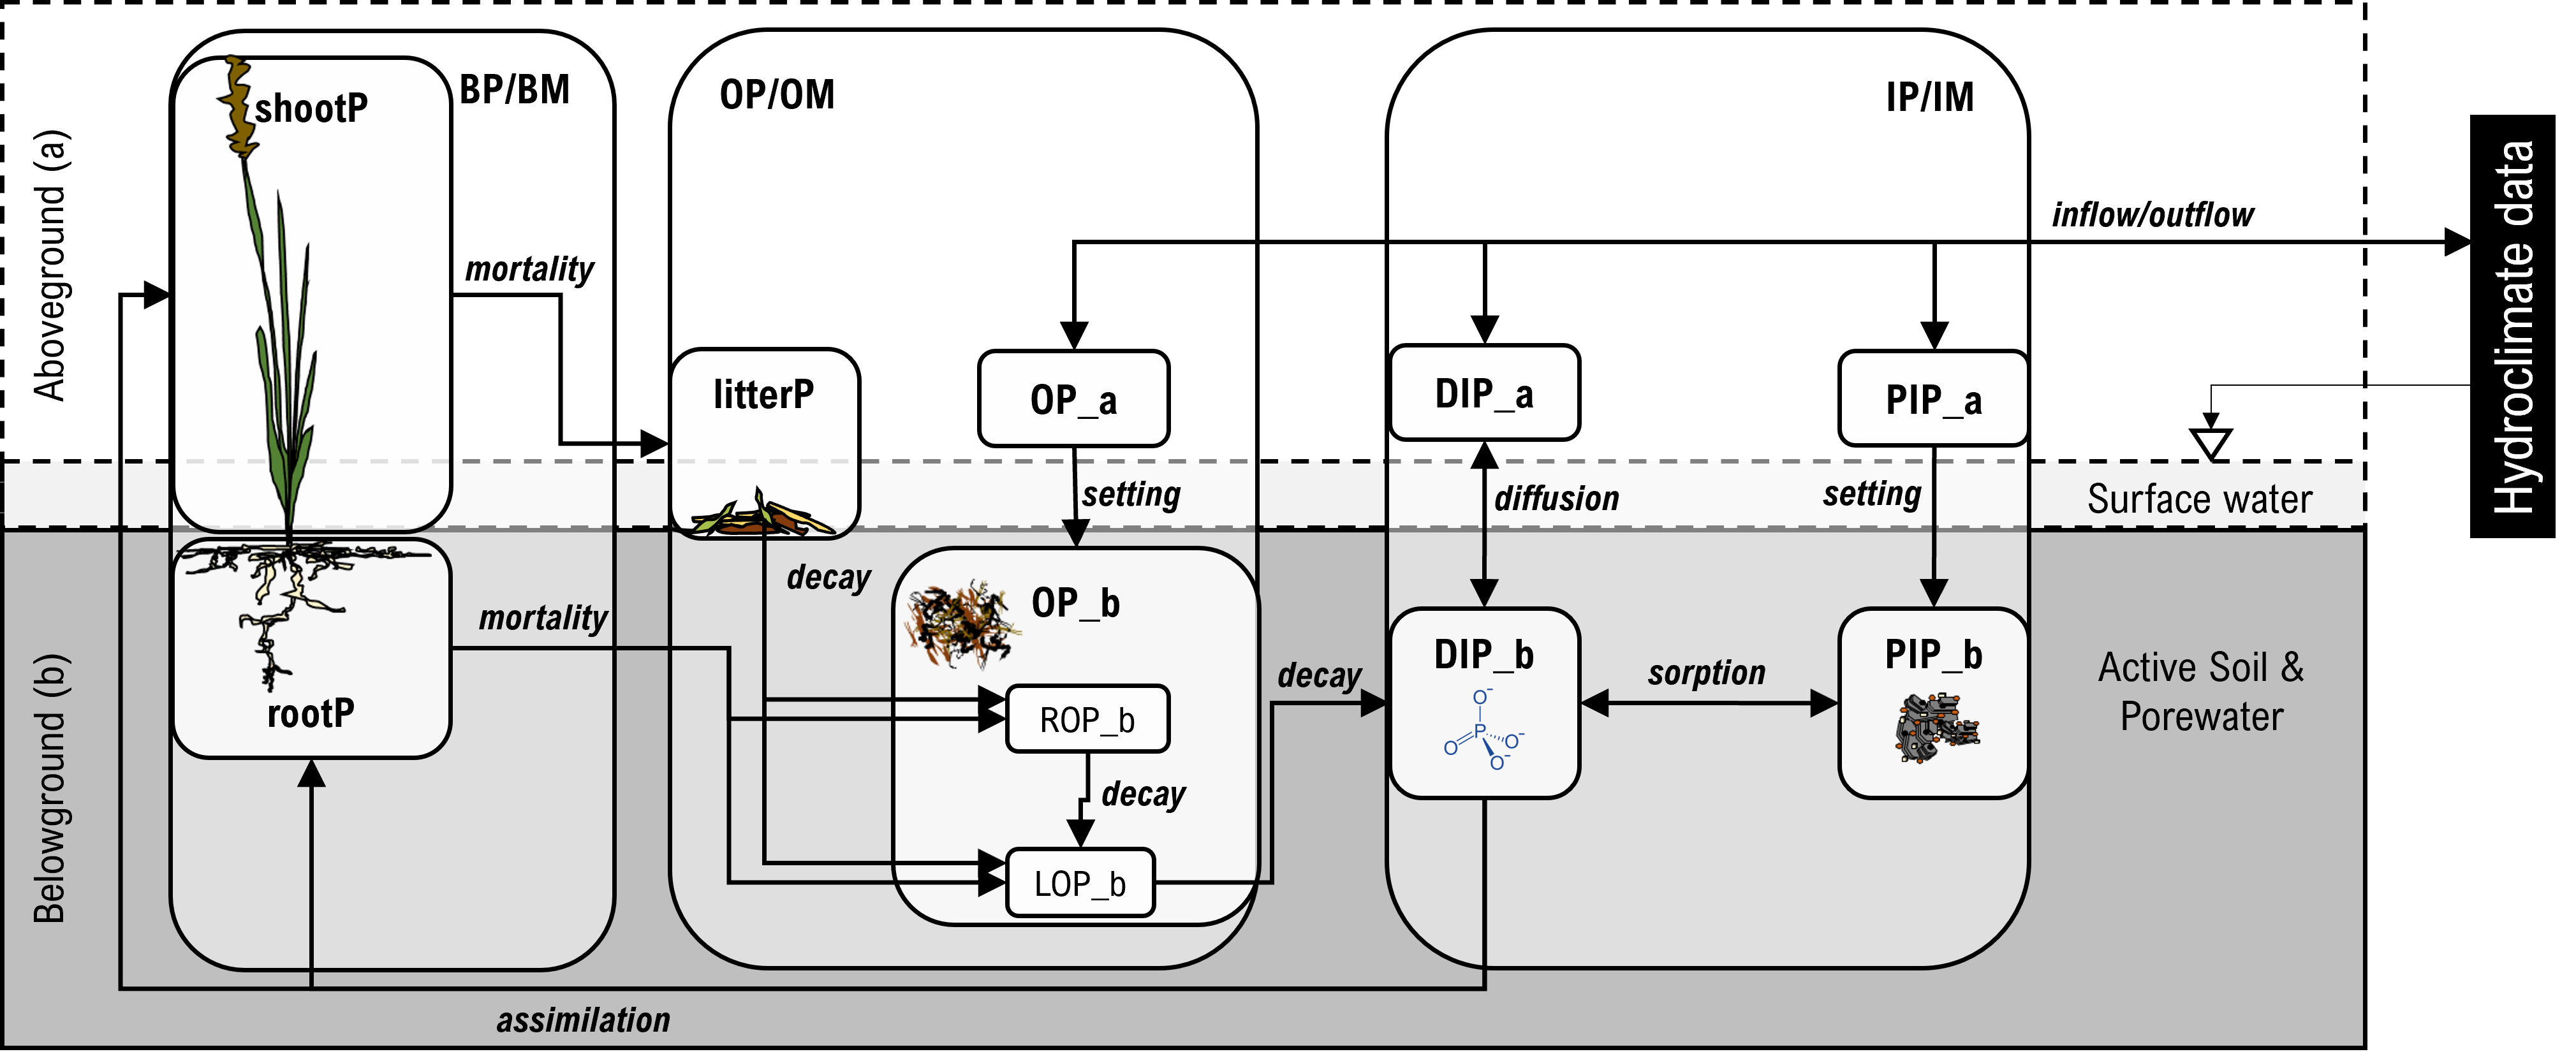
\includegraphics{C:/Users/Adrian.Wiegman/Documents/GitHub/wetlandP_2p1_stable/wetlandP_v2.1/documentation/wetlandP_v2.1_Conceptual_Diagram.png}

The figure below shows a time series plot of the model state variables.

\includegraphics{ReadMe_files/figure-latex/unnamed-chunk-9-1.pdf}

The default parameters for wetlandP\_v2.1 currently produce state
variable values close to what has been observed in the field. This
includes dissolved inorganic P concentrations (see plot below)

\includegraphics{ReadMe_files/figure-latex/unnamed-chunk-10-1.pdf}

\hypertarget{state-variables}{%
\subsubsection{State variables}\label{state-variables}}

\begin{longtable}[]{@{}lll@{}}
\caption{state variables calculated with ordinary differential
equations}\tabularnewline
\toprule\noalign{}
name & unit & description \\
\midrule\noalign{}
\endfirsthead
\toprule\noalign{}
name & unit & description \\
\midrule\noalign{}
\endhead
\bottomrule\noalign{}
\endlastfoot
IM\_a & g d.w & inorganic matter aboveground \\
IM\_b & g d.w & inorganic matter belowground \\
shootP & g P & aboveground live shoot P \\
rootP & g P & belowground live root P \\
litterP & g P & aboveground litter P \\
ROP\_a & g P & refractory OP aboveground \\
LOP\_a & g P & labile OP aboveground \\
PIP\_a & g P & particulate IP aboveground \\
DIP\_a & g P & dissolved IP aboveground \\
ROP\_b & g P & refractory OP belowground \\
LOP\_b & g P & labile OP belowground \\
PIP\_b & g P & particulate IP belowground \\
DIP\_b & g P & dissolved IP belowground \\
\end{longtable}

\hypertarget{processes}{%
\subsubsection{Processes}\label{processes}}

\hypertarget{flows}{%
\paragraph{Flows}\label{flows}}

\begin{longtable}[]{@{}lllll@{}}
\caption{process flows (adding or subtracting from state
variables)}\tabularnewline
\toprule\noalign{}
Name & Value & Unit & Description & Assumptions \\
\midrule\noalign{}
\endfirsthead
\toprule\noalign{}
Name & Value & Unit & Description & Assumptions \\
\midrule\noalign{}
\endhead
\bottomrule\noalign{}
\endlastfoot
Q\_in & IO\_Q\_in*Q\_in & m\^{}3/d & surface water lateral inflow & note
all hydrologic should be positive magnitude values, they are then
multiplied by 1, 0, -1 in differential equaitions \\
Q\_out & IO\_Q\_out*Q\_out & m\^{}3/d & surface water lateral outflow
& \\
Q\_ground & IO\_Q\_ground*Q\_ground & m\^{}3/d & net vertical flow from
groundwater (percolation - infiltration) & \\
Q\_precip & IO\_Q\_precip*Q\_precip & m\^{}3/d & direct precipitation
& \\
Q\_ET & IO\_Q\_ET*Q\_ET & m\^{}3/d & evapotranspiration precipitation
& \\
assim\_shootP & IO\_assim\_shootP*r\_assim*BM*k\_BM2P*k\_f\_G\_shoot & g
P/d & assimilation of shoot P & \\
assim\_rootP & IO\_assim\_rootP*r\_assim*BM*k\_BM2P*(1-k\_f\_G\_shoot) &
g P/d & growth of root P & \\
mort\_shootP2litterP & IO\_mort\_shootP2litterP*r\_mort\_shoot*shootP &
g P/d & growth of root P & \\
mort\_rootP2LOP &
IO\_mort\_rootP2LOP*r\_mort\_root*rootP*(k\_f\_labile\_root) & g P/d &
mortality of shoot P to LOP & \\
mort\_rootP2ROP &
IO\_mort\_rootP2ROP*r\_mort\_root*rootP*(1-k\_f\_labile\_root) & g P/d &
mortatlity of root P & \\
sed\_IM & IO\_sed\_IM*r\_sed\_IM*IM\_a & g d.w./d & sedimentation of
inorganic matter & \\
sed\_PIP & IO\_sed\_IM*r\_sed\_IM*PIP\_a & g P/d & sedimentation of
inorganic P & \\
sed\_LOP & IO\_sed\_OM*r\_sed\_OM*LOP\_a & g P/d & sedimentation of
labile organic P & \\
sed\_ROP & IO\_sed\_OM*r\_sed\_OM*ROP\_a & g P/d & sedimentation of
refractory organic P & \\
dec\_litter2LOP\_a &
IO\_decay\_litter*r\_decay\_litter*litterP*(k\_f\_labile\_litter) & &
decomposition of litter P to labile organic P & \\
dec\_litter2ROP\_a &
IO\_decay\_litter*r\_decay\_litter*litterP*(1-k\_f\_labile\_litter) & &
decomposition of litter P to refractory organic P & \\
dec\_LOP\_a & IO\_decay\_LOP*r\_decay\_LOP*LOP\_a & g P/d &
decomposition of labile OP to DIP & \\
dec\_ROP\_a & IO\_decay\_ROP*r\_decay\_ROP*ROP\_a & g P/d &
decomposition of refractory OP to labile OP & \\
dec\_LOP\_b & IO\_decay\_LOP*r\_decay\_LOP*LOP\_b & g P/d &
decomposition of labile OP to DIP & \\
dec\_ROP\_b & IO\_decay\_ROP*r\_decay\_ROP*ROP\_b & g P/d &
decomposition of refractory OP to labile OP & \\
diff\_DIP\_b2a & IO\_diffus*r\_diffus*DIP\_b & g P/d & diffusion of DIP
from b to a & \\
sorp\_DIP2PIP\_b & IO\_adsorp*r\_adsorp*V\_w\_b & g P/d & adsorption of
DIP onto PIP & \\
in\_IM & IO\_in\_IM*Q\_in*ISS & g d.w./d & inflow of inorganic matter as
ISS & \\
in\_PIP & IO\_in\_PIP*(in\_IM*k\_ISS2P + Q\_in*SRP*k\_SRP2PIP) & g P/d &
inflow of PIP & \\
in\_LOP & IO\_in\_LOP*Q\_in*OSS*k\_BM2P*(k\_f\_labile) & g P/d & inflow
of labile organic P & \\
in\_ROP & IO\_in\_ROP*Q\_in*OSS*k\_BM2P*(1-k\_f\_labile) & g P/d &
inflow of recalcitrant organic P & \\
in\_DIP & IO\_in\_DIP*Q\_in*SRP & g P/d & inflow of dissolved inorganic
P & \\
out\_IM & IO\_out\_IM*Q\_out*IM\_a/V\_w\_a & g P/d & outflow of IM & \\
out\_PIP & IO\_out\_PIP*Q\_out*PIP\_a/V\_w\_a & g P/d & outflow of PIP
& \\
out\_LOP & IO\_out\_LOP*Q\_out*LOP\_a/V\_w\_a & g P/d & outflow of LOP
& \\
out\_ROP & IO\_out\_ROP*Q\_out*ROP\_a/V\_w\_a & g P/d & outflow of ROP
& \\
out\_DIP & IO\_out\_DIP*Q\_out*DIP\_a/V\_w\_a & g P/d & outflow of DIP
& \\
\end{longtable}

\hypertarget{rates}{%
\paragraph{Rates}\label{rates}}

\begin{longtable}[]{@{}llll@{}}
\caption{process rates (calculated as a function of forcing variables,
intermediate variables and state variables)}\tabularnewline
\toprule\noalign{}
name & unit & description & assumptions \\
\midrule\noalign{}
\endfirsthead
\toprule\noalign{}
name & unit & description & assumptions \\
\midrule\noalign{}
\endhead
\bottomrule\noalign{}
\endlastfoot
r\_assim & g P/d & amount of DIP\_b P (g) assimilated by macrophyte
plants as net primary productivity & always affected by temperature, DIP
availability, and optionally affected by water level, and self-crowding
or shading (Marois \& Mitsch 2016; Morris et al.~2002; Wiegman et
al.~2019) \\
r\_decay\_litter & 1/d & proportional rate of litter decomposition &
affected by temperature (Wang et al.~2003) \\
r\_decay\_ROP & 1/d & proportional rate of ROP decomposition & same as
r\_decay\_litter \\
r\_decay\_LOP & 1/d & proportional rate of LOP decomposition & same as
r\_decay\_litter \\
r\_mort\_shoot & 1/d & proportional rate of shoot death & affected by
temperature, increases as a step function when temp drops below
threshold (based on field observations) (Wiegman et al.~2019) \\
r\_mort\_root & 1/d & proportional rate of root death & affected by
temperature (Morris et al.~2002) \\
r\_adsorp\_b & g P/d & ammount of DIP adsorbed to PIP belowground &
affected by temperature and equilibrium DIP (Wang et al.~2003);
equilibrium DIP can be set as a parameter, or calculated as a function
from maximum P storage capacity (Ex\_max, variable or constant), and the
currently adsorbed P (Ex = PIP\_b). \\
r\_diffus & g P/d & amount of diffusion of DIP\_b to DIP\_a & affected
by temperature, viscosity of water, concentration gradient, distance,
and tortuosity of fluid matrix (Wang et al.~2003; Reddy \& Delaune
2008) \\
r\_sed\_IM & 1/d & proportional rate of sedimentation of IM\_a to IM\_b
& affected by settling velocity (temperature, viscosity of water,
particle radius, particle density) and water depth, set equal to 1 when
depth is less than settling velocity (Reddy \& Delaune 2008) \\
r\_sed\_OM & 1/d & proportional rate of sedimentation of OM\_a to OM\_b
& same as r\_sed\_OM \\
\end{longtable}

\hypertarget{forcings-hydroclimatic-inputs}{%
\subsubsection{Forcings (Hydroclimatic
Inputs)}\label{forcings-hydroclimatic-inputs}}

The table below gives the variable names and assumptions for the forcing
variables used in the model. The model was forced with water level data
collected in situ and meteorological data from Burlington Int'l Airport
(NOAA NCDC). Water level was measured at field sites by HOBO MX2001
pressure and temperature sensors placed just below the soil surface.
Data was corrected for variation in local barometric pressure, also
measured by HOBO MX2001s. Any gaps in the water level sensor record were
filled via time lag regression with other sensors in the area or with
USGS guages (USGS NWIS, r\^{}2\textgreater0.9). Water temperature was
modeled from air temperature based using a statistical fit to with
miniDOT sensors at the soil water interface (r\^{}2\textgreater0.9).
Precipitation was taken as the daily totals from meteorological data.
Evapotranspiration rate was estimated using the penman monteith method
via the R package \texttt{evapotranspiration}, substituting sunshine
hours for solar radiation. Water volume were calculated from area,
porosity (assumed = 1), and water depth. We caclulated the first
derivative in the time of water volume, and used this to solve for net
surface flow. Surface inflow and outflow were deduced from net surface
flow by adjusting for through flow. Through flow was calculated as the
volume of water divided by the days hydraulic residence time (HRT or
\(\tau\)).

\$\$

\text{HYDROLOGY SUBROUTINE:}\textbackslash{} V\_w =
A\rho\emph{aH\_w\textbackslash{} dV}\{w\} = V\_\{w,t\} - V\_\{w,t+1\}
\textbackslash{} Q\_\{net\}= dV\_w - A(ip - ET) \textbackslash{}
\text{IF Q}\emph{\text{net} \textgreater{} 0: \textbackslash{} Q}\{in\}
= Vw/\tau + Qnet \textbackslash{} Q\_\{in\} = -
V\_w/\tau \textbackslash{} \text{ELSE:} \textbackslash{} Q\_\{in\} =
V\_w/\tau \textbackslash{} Q\_\{out\} = V\_w/\tau - Q\_\{net\}
\textbackslash{}

\$\$

\begin{verbatim}
## Warning: One or more parsing issues, call `problems()` on your data frame for details,
## e.g.:
##   dat <- vroom(...)
##   problems(dat)
\end{verbatim}

\begin{verbatim}
## Rows: 14 Columns: 4
## -- Column specification --------------------------------------------------------
## Delimiter: "|"
## chr (4): Symbol ,  Units ,  Definition ,  Assumptions and Sources
## 
## i Use `spec()` to retrieve the full column specification for this data.
## i Specify the column types or set `show_col_types = FALSE` to quiet this message.
\end{verbatim}

\begin{longtable}[]{@{}lccc@{}}
\caption{Table 1. Hydroclimate variables}\tabularnewline
\toprule\noalign{}
Symbol & Units & Definition & Assumptions and Sources \\
\midrule\noalign{}
\endfirsthead
\toprule\noalign{}
Symbol & Units & Definition & Assumptions and Sources \\
\midrule\noalign{}
\endhead
\bottomrule\noalign{}
\endlastfoot
Zs & (m, NAD'83) & elevation of sediment surface & estimated from LiDAR
0.5m DEM (VCGI), corrected with Emlid Reach RS+ RTK/GNSS survey
(centimeter level accuracy) \\
Hw & (m) & height of water above sediment surface & measured with HOBO
MX2001 water level logger \\
Zw & (m, NAD'83) & elevation of water & Hw + Zs \\
A & (m\^{}2) & wetland surface area & interpolated from stage table as
f(Hw) \\
Vw & (m\^{}3) & Water volume of wetland surface water & calculated from
A and H\_w \\
ET & (cm/day) & Evapotranspiration rate & Calculated at daily intervals
with penman monteith equation via the \texttt{Evapotranspiration}
package, weather data from BURLINGTON INTERNATIONAL AIRPORT, VT US
(WBAN:14742) (NOAA NCDC) \\
ip & (cm/day) & Precipitation rate & totals derived from sub-hourly
weather observations from BURLINGTON INTERNATIONAL AIRPORT, VT US
(WBAN:14742)(NOAA NCDC) \\
Qnet & (m\^{}3) & net surface flow & deduced from dVw, and A(ip - ET) \\
Qin & (m\^{}3/day) & Volumetric inflow rate & modeled with HydroCAD
and/or solved from water balance \\
Qout & (m\^{}3/day) & Wetland discharge (outflow) rate & Modeled as a
f(Hw) based on site observations \\
Qg & (m\^{}3/day) & Groundwater discharge (negative for infiltration) &
assumed = 0 \\
Uw & (m/s) & Wind speed & mean derived from sub-hourly data from
BURLINGTON INTERNATIONAL AIRPORT, VT US (WBAN:14742) \textbar{} used in
evapotranspiration calculation \\
Tair & (°C) & Daily air temperature & mean derived from sub-hourly data
BURLINGTON INTERNATIONAL AIRPORT, VT US (WBAN:14742) \textbar{} \\
TW & (°C) & Daily water average temperature & Modeled from Tair using
equation from linear model fit to temperature measured with PME miniDOT.
IF(Tair \textgreater{} 0): TW = 2.5+0.8Tair ELSE: TW = 0 \\
\end{longtable}

\hypertarget{parameters}{%
\subsubsection{Parameters}\label{parameters}}

\begin{longtable}[]{@{}lllll@{}}
\caption{local (measured) parameters}\tabularnewline
\toprule\noalign{}
Name & Value & Unit & Description & Assumptions \\
\midrule\noalign{}
\endfirsthead
\toprule\noalign{}
Name & Value & Unit & Description & Assumptions \\
\midrule\noalign{}
\endhead
\bottomrule\noalign{}
\endlastfoot
area & 1 & m\^{}2 & wetland surface area & uniform flat surface \\
H\_b & 0.1 & m & height of belowground compartment (sediment column) &
NA \\
k\_HRT & 1e3 & d & hydraulic residence time of wetland surface water &
calculated by dividing total system water volume (m3) by outlfow rate
(m3/d), often changes as function of system water volume \\
k\_TSS & 15 & g/m\^{}3 & total suspended solids of inflow & based on
field data, median of observations, 3.5 at prindle, 23.8 at union st,
12.25 at swamp rd \\
k\_TP & 0.05 & g P/m\^{}3 & TP concentration (mg P /L) in inflow & 0.071
at prindle, 0.059 at union, 0.056 at swamp \\
k\_LOI & 0.20 & g/g & initial fraction of organic matter in total mass
of below ground compartment & measured as soil loss-on-ignition \\
k\_PSR & 0.20 & mol/mol & P Saturation Ratio & molar ratio of oxalate
extractable P/(Al + Fe) (Nair et al.~2004), fit to field data, prindle
0.09 - 0.15, union 0.08 - 0.13, swamp rd 0.11 - 0.26 \\
k\_Ex\_max & 4 & g/kg & maximum P storage capacity & 31*(Al/27 + Fe/56),
where Al and Fe are determined by acid ammonium oxalate extraction, fit
to field data, ranging from 3.3 - 5.5 prindle, 5.0 - 6.4 union, 3.44 -
5.1 swamp \\
k\_clay & 0.1 & g/g & clay content of inorganic matter, used for
particle settling velocity & from soil textural analysis OR from NRCS
soil survey units texture class, .11 to 0.35, .0875 to 0.15 union, 0.075
- .15 swamp \\
k\_f\_fines & 0.90 & g/g & silt + clay, fine sediment fraction of
incoming total suspended solids used for particle setting velocity & fit
to field data and 0.627 - .84 prindle, 0.84 - 0.97 union, 0.75 - 0.985
swamp rd. \\
k\_f\_OSS & 0.5 & g/g & organic matter fraction of incoming total
suspended solids & fit to field data, \%65 at prindle rd, 23\% at union
st, 54\% swamp rd. \\
k\_f\_SRP & 0.3 & g SRP /g TP & fraction of TP as SRP in influent water
& based on field data 0.404 at prindle, 0.25 at union, 0.27 at swamp
rd. \\
k\_DIP\_E & 0.05 & & equilibrium DIP concentration & used if
IO\_variable\_DIP\_E = F, set equal to final intact SRP for aerobic
treatments \\
k\_rp\_i & fn\_particle\_radius(sand & & average radius of inorganic
particles & calculated based on soil texture see
\texttt{fn\_particle\_radius} \\
\end{longtable}

\begin{longtable}[]{@{}lllll@{}}
\caption{stochastic (unmeasured/calibrated) parameters}\tabularnewline
\toprule\noalign{}
Name & Value & Unit & Description & Assumptions \\
\midrule\noalign{}
\endfirsthead
\toprule\noalign{}
Name & Value & Unit & Description & Assumptions \\
\midrule\noalign{}
\endhead
\bottomrule\noalign{}
\endlastfoot
k\_T\_STD & 13.75 & deg C & standard temperature for metabolic processes
& calibrated to make actual NPP match ANPPmax, since experiments were
conducted under field conditions this parameter is equal to the (maximum
daily average temp - minimum daily average temp)/2 + minimum daily
average temp \textasciitilde{} 15 - 17 degrees \\
k\_SRP2PIP & 0.98 & g P/d.w. & ratio of LOP to SRP & 8.9e-1 for prindle,
1.42 for swamp rd, 6.2e-1 for union st \\
k\_ISS2P & 0.0013 & g P/d.w. & P content of inorganic suspended
sediments & site data 0.002 for prindle rd, 0.0009 for union st, 0.00094
for swamp rd \\
k\_shootM & 0 & g dw/m2 & shoot live biomass & need to set up a way to
get this to vary based on start time \\
k\_rootM & 1000 & g dw/m2 & shoot live biomass & need to set up a way to
get this to vary based on start time \\
k\_BM2P & 0.001 & g/g P/d.w. & P content of biomass & McJannet et
al.~1996 .001 - 0.003; Morris \& Bowden 1986 0.002; Wiegman Ch 2 data
0.001 to 0.003 \\
k\_f\_G\_shoot & 0.5 & fraction & fraction of NPP allocated to shoot
growth (shoot\_NPP/total\_NPP) & Morris et al 1984 0.2 - 0.5 \\
k\_NPP & 1500 & g m-2 y-1 & combined annual rate of NPP for above and
below ground biomass & Morris et al.~1984 1000 to 4000 \\
k\_ADNPP & k\_NPP/365 & g m-2 d-1 & average daily rate of NPP & divide
k\_NPP by 365 \\
k\_M & 0.001 & 1/day & rate of baseline biomass mortality & calibrated
to root mass \textasciitilde1000 - 2000 g m-2 and peak shootM
\textasciitilde300-800 g m-2 at use 0.003 for k\_ANPPmax = 3000, with
guidance from Morris et al 1984 0.003 to 0.007; Marois \& Mitsch 2016
0.0005 - 0.007 \\
k\_M\_shoot\_T\_mult & 50 & factor & multiplier for shoot mortality
after temp drops below threshold & calibrated to field observations \\
k\_T\_thresh\_M\_shoot & 6 & deg C & temperature at which shoot
mortality increases & calibrated to field observations \\
k\_whc & 1e-3 & & a small volume of water to prevent errors associated
with empty compartments & best guess based on fit of oven dry verses air
dry moisture content \\
k\_diff\_STD & 1e-1 & m\^{}2/d & effective diffusion coefficient &
calibrated to intact core data; Marois \& Mitsch 2016 calibrated value
was 2e−5 m2 d−1 \\
k\_ad & 1.75 & 1/d & adsorption first order rate coefficient & Wang et
al.~2003 1.75, Marois \& Mitsch 2016 used \\
k\_E & .56 & m\^{}3/g & langmuir constant of adsorption (bond energy) &
Calibrated to intact core data this value depends on what metric is used
to define Ex\_max, Wang et al.~2003 2.75 m3 kg-1 \\
k\_PIP2Ex & 1 & g/g & ratio of exchangeable P to particulate inorganic P
& Wang et al.~2003 0.8 \\
k\_f\_labile & 0.8 & g/g & labile fraction organic matter & Morris \&
Bowden 1986 refractory fraction of 0.2 k\_f\_LOM\_OSS = k\_f\_labile \#
g/g \\
k\_decay\_litter & 0.01 & 1/d & litter decomposition rate coefficient at
STD temp & Morris \& Bowden, Wiegman Ch 3, \# Longhi et al.~2008 k =
ranged from 0.01 1/d to 0.0027 1/d \\
k\_decay\_LOP & 0.01 & 1/d & LOP decomposition rate coefficient at STD
temp & Marois \& Mitsch 2016 DOP rate is 0.01, while LPOP rate is 0.003,
since we do not model DOP LOP decay should be between 0.001 - 0.01 \\
k\_decay\_ROP & 1e-5 & 1/d & ROP decomposition rate coefficient at STD
temp when soils are unsaturated and aerobic(H\_w \textless{} 0) & Morris
\& Bowden 1986 assume refractory OM does not decompose, however this is
assuming saturated soils, so we assume that when H\_w \textless{} 0 that
ROP decomposes at between 1e-5 and 5e-5 based on value from Marois \&
Mitsch 2016 of 2.5e-5 \\
k\_rp\_o & 4.5e-7 & m & average radius of organic particles & Marois \&
Mitsch 2016 \\
\end{longtable}

\begin{longtable}[]{@{}lllll@{}}
\caption{universal constant parameters}\tabularnewline
\toprule\noalign{}
Name & Value & Unit & Description & Assumptions \\
\midrule\noalign{}
\endfirsthead
\toprule\noalign{}
Name & Value & Unit & Description & Assumptions \\
\midrule\noalign{}
\endhead
\bottomrule\noalign{}
\endlastfoot
k\_dp\_i & 2.65e6 & g/m\^{}3 & particle density of inorganic matter &
Delaune et al.~1983 g/cm\^{}3 * 10\^{}6 cm\textsuperscript{3/m}3 \\
k\_dp\_o & 1.14e6 & g/m\^{}3 & particle density of inorganic matter &
Delaune et al.~1983 g/cm\^{}3 * 10\^{}6 cm\textsuperscript{3/m}3 \\
k\_db\_i & 1.99e6 & g/m\^{}3 & bulk density of inorganic matter & Morris
et al.~2016 \\
k\_db\_o & 0.085e6 & g/m\^{}3 & bulk density of organic matter & Morris
et al.~2016 \\
k\_pi & 3.141593 & & arc length of a circle & \\
k\_g & 7.32e10 & m/d\^{}2 & acceleration due to gravity & constant \\
k\_mew & 86.4e3 & g/m/d & viscosity of water & standard value \\
k\_dw & 1e6 & g/m\^{}3 & density of water & 1e6 for 0 salinity, 1.025e6
for 34 ppm salinity water \\
k\_diff & 1.931741e-05 & m\^{}2/d & effective diffusion coefficient &
standard tempurature and pressure see fn\_kDiff \\
\end{longtable}

\begin{longtable}[]{@{}lllll@{}}
\caption{run specifications parameters}\tabularnewline
\toprule\noalign{}
Name & Value & Unit & Description & Assumptions \\
\midrule\noalign{}
\endfirsthead
\toprule\noalign{}
Name & Value & Unit & Description & Assumptions \\
\midrule\noalign{}
\endhead
\bottomrule\noalign{}
\endlastfoot
version & ``wetlandPv02'' & chr & name of the model version & \\
simname & ``default'' & chr & name of the model simulation & \\
simtype & ``static'' & chr & charater string indicating the objective of
the model run used & ``static'' for steady sate, ``forecast'' for
projections and scenario analysis, and ``calibration'' for
training/calibration \\
startday & 0 & d & julian day (0-365) of simulation start & based period
of forcing data \\
simyears & 14/365 & y & number of years in simulation & ``\,'' \\
increment & 1 & d & number of days in each time step of model & if not
equal to 1 then accuracy of simulation needs to be verified \\
extended\_outputs & T & logical & True/False indicating if the purpose
of the run is to debug & if so writes extended outputs, this
significantly slows the run time \\
IO\_Q\_in & T & logical & toggles surface inflow & T/F or 1/0 \\
IO\_Q\_precip & T & logical & toggle precipitation & \\
IO\_Q\_ground & T & logical & toggles net groundwater flow (percolation
- infiltration) & \\
IO\_Q\_ET & T & logical & toggles evapotranspiration & \\
IO\_Q\_out & T & logical & toggles surface outflow & \\
IO\_assim\_shootP & T & logical & toggles assimilation of shoot P & \\
IO\_assim\_rootP & T & logical & toggles growth of root P & \\
IO\_mort\_shootP2litterP & T & logical & toggles mortality of shoots
& \\
IO\_mort\_rootP2LOP & T & logical & toggles mortality of root P to LOP
& \\
IO\_mort\_rootP2ROP & T & logical & toggles mortatlity of root P & \\
IO\_sed\_IM & T & logical & toggles sedimentation of inorganic matter
& \\
IO\_decay\_litter & T & logical & toggles decomposition of litter P to
refractory organic P & \\
IO\_decay\_LOP & T & logical & toggles decomposition of labile OP & \\
IO\_decay\_ROP & T & logical & toggles decomposition of refractory OP
& \\
IO\_diffus & T & logical & toggles diffusion of DIP from b to a & \\
IO\_adsorp & T & logical & toggles adsorption of DIP onto PIP & \\
IO\_in\_IM & T & logical & toggles inflow of inorganic matter as ISS
& \\
IO\_in\_PIP & T & logical & toggles inflow of PIP & \\
IO\_in\_LOP & T & logical & toggles inflow of labile organic P & \\
IO\_in\_ROP & T & logical & toggles inflow of recalcitrant organic P
& \\
IO\_in\_DIP & T & logical & toggles inflow of dissolved inorganic P & \\
IO\_out\_IM & T & logical & toggles outflow of IM & \\
IO\_out\_PIP & T & logical & toggles outflow of PIP & \\
IO\_out\_LOP & T & logical & toggles outflow of LOP & \\
IO\_out\_ROP & T & logical & toggles outflow of ROP & \\
IO\_out\_DIP & T & logical & toggles outflow of DIP & \\
IO\_DIP\_E\_langmuir & F & logical & turns on the use of langmuir model
for caclulating DIP\_E & \\
IO\_variable\_k\_E & T & logical & toggles variable calculation of k\_E
& \\
IO\_variable\_k\_Ex\_max & F & logical & toggles on variable calculation
of Ex\_max using statistical fit to fines and LOI & \\
IO\_anoxic & F & logical & toggles anaerobic conditions for DIP\_E
concentration & \\
IO\_variable\_DIP\_E & F & logical & toggles variable calculation of
DIP\_E & if = F, then k\_DIP\_E is used \\
IO\_Q\_net & T & logical & toggles calculation of inflow and outflow
from Qnet, Vw and HRT & see hydrology subroutine \\
IO\_HRT\_power\_model & F & logical & toggles calculation HRT from a
power model & if Zw \textgreater{} 0, HRT = a*Zw\^{}b, where Zw is
elevation relative to lowest elevation in the wetland, and
b\textless0 \\
\end{longtable}

\hypertarget{differential-equations}{%
\subsubsection{Differential Equations}\label{differential-equations}}

Differential Equations for the model are generated from stoicheometry
matrix of the \textbf{state variables} and \textbf{process flows} (see
\textbf{``mass balance''}).

\begin{longtable}[]{@{}ll@{}}
\caption{Differential equations for model states}\tabularnewline
\toprule\noalign{}
Name & Value \\
\midrule\noalign{}
\endfirsthead
\toprule\noalign{}
Name & Value \\
\midrule\noalign{}
\endhead
\bottomrule\noalign{}
\endlastfoot
d\_IM\_a & -1 * sed\_IM + 1 * in\_IM + -1 * out\_IM \\
d\_IM\_b & 1 * sed\_IM \\
d\_shootP & 1 * assim\_shootP + -1 * mort\_shootP2litterP \\
d\_rootP & 1 * assim\_rootP + -1 * mort\_rootP2LOP + -1 *
mort\_rootP2ROP \\
d\_litterP & 1 * mort\_shootP2litterP + -1 * dec\_litter2LOP\_a + -1 *
dec\_litter2ROP\_a \\
d\_ROP\_a & -1 * sed\_ROP + 1 * dec\_litter2ROP\_a + -1 * dec\_ROP\_a +
1 * in\_ROP + -1 * out\_ROP \\
d\_LOP\_a & -1 * sed\_LOP + 1 * dec\_litter2LOP\_a + -1 * dec\_LOP\_a +
1 * dec\_ROP\_a + 1 * in\_LOP + -1 * out\_LOP \\
d\_PIP\_a & -1 * sed\_PIP + 1 * in\_PIP + -1 * out\_PIP \\
d\_DIP\_a & 1 * dec\_LOP\_a + 1 * diff\_DIP\_b2a + 1 * in\_DIP + -1 *
out\_DIP \\
d\_ROP\_b & 1 * mort\_rootP2ROP + 1 * sed\_ROP + -1 * dec\_ROP\_b \\
d\_LOP\_b & 1 * mort\_rootP2LOP + 1 * sed\_LOP + -1 * dec\_LOP\_b + 1 *
dec\_ROP\_b \\
d\_PIP\_b & 1 * sed\_PIP + 1 * sorp\_DIP2PIP\_b \\
d\_DIP\_b & -1 * assim\_shootP + -1 * assim\_rootP + 1 * dec\_LOP\_b +
-1 * diff\_DIP\_b2a + -1 * sorp\_DIP2PIP\_b \\
\end{longtable}

\hypertarget{mass-balance}{%
\subsubsection{Mass balance}\label{mass-balance}}

Differential Equations for the model are generated from stoicheometry
matrix of the \textbf{state variables} (state or states for short) and
\textbf{process flows} (see \texttt{stoicheometry.xlsx}). In this matrix
the modeler enters a value of 1 (adding to a state), -1 (subtracting
from state) or blank (not interacting with a state) for each combination
of a state variable and a process flow. The table below contains the
stoicheometry matrix for the current model. Note the column
\texttt{balance} is the row sum for a given process, values above or
below than zero indicates that a process adds/removes mass from the
model domain, while a balance of zero indicates that a process is
conservative (does not affect the total mass in the domain).

\begin{longtable}[]{@{}rlrrrrrrrrrrrrr@{}}
\caption{parameters (numeric constants and run
specifications)}\tabularnewline
\toprule\noalign{}
balance & variables (right) processes (below) & IM\_a & IM\_b & shootP &
rootP & litterP & ROP\_a & LOP\_a & PIP\_a & DIP\_a & ROP\_b & LOP\_b &
PIP\_b & DIP\_b \\
\midrule\noalign{}
\endfirsthead
\toprule\noalign{}
balance & variables (right) processes (below) & IM\_a & IM\_b & shootP &
rootP & litterP & ROP\_a & LOP\_a & PIP\_a & DIP\_a & ROP\_b & LOP\_b &
PIP\_b & DIP\_b \\
\midrule\noalign{}
\endhead
\bottomrule\noalign{}
\endlastfoot
0 & assim\_shootP & & & 1 & & & & & & & & & & -1 \\
0 & assim\_rootP & & & & 1 & & & & & & & & & -1 \\
0 & mort\_shootP2litterP & & & -1 & & 1 & & & & & & & & \\
0 & mort\_rootP2LOP & & & & -1 & & & & & & & 1 & & \\
0 & mort\_rootP2ROP & & & & -1 & & & & & & 1 & & & \\
0 & sed\_IM & -1 & 1 & & & & & & & & & & & \\
0 & sed\_PIP & & & & & & & & -1 & & & & 1 & \\
0 & sed\_LOP & & & & & & & -1 & & & & 1 & & \\
0 & sed\_ROP & & & & & & -1 & & & & 1 & & & \\
0 & dec\_litter2LOP\_a & & & & & -1 & & 1 & & & & & & \\
0 & dec\_litter2ROP\_a & & & & & -1 & 1 & & & & & & & \\
0 & dec\_LOP\_a & & & & & & & -1 & & 1 & & & & \\
0 & dec\_ROP\_a & & & & & & -1 & 1 & & & & & & \\
0 & dec\_LOP\_b & & & & & & & & & & & -1 & & 1 \\
0 & dec\_ROP\_b & & & & & & & & & & -1 & 1 & & \\
0 & diff\_DIP\_b2a & & & & & & & & & 1 & & & & -1 \\
0 & sorp\_DIP2PIP\_b & & & & & & & & & & & & 1 & -1 \\
1 & in\_IM & 1 & & & & & & & & & & & & \\
1 & in\_PIP & & & & & & & & 1 & & & & & \\
1 & in\_LOP & & & & & & & 1 & & & & & & \\
1 & in\_ROP & & & & & & 1 & & & & & & & \\
1 & in\_DIP & & & & & & & & & 1 & & & & \\
-1 & out\_IM & -1 & & & & & & & & & & & & \\
-1 & out\_PIP & & & & & & & & -1 & & & & & \\
-1 & out\_LOP & & & & & & & -1 & & & & & & \\
-1 & out\_ROP & & & & & & -1 & & & & & & & \\
-1 & out\_DIP & & & & & & & & & -1 & & & & \\
\end{longtable}

\hypertarget{numerical-stability-checks}{%
\subsubsection{Numerical Stability
Checks}\label{numerical-stability-checks}}

The following figures verify the performance of the model under
increasing complexity of simulation.

\hypertarget{all-stocks-should-be-constant-through-time}{%
\paragraph{1. all stocks should be constant through
time}\label{all-stocks-should-be-constant-through-time}}

\begin{figure}
\centering
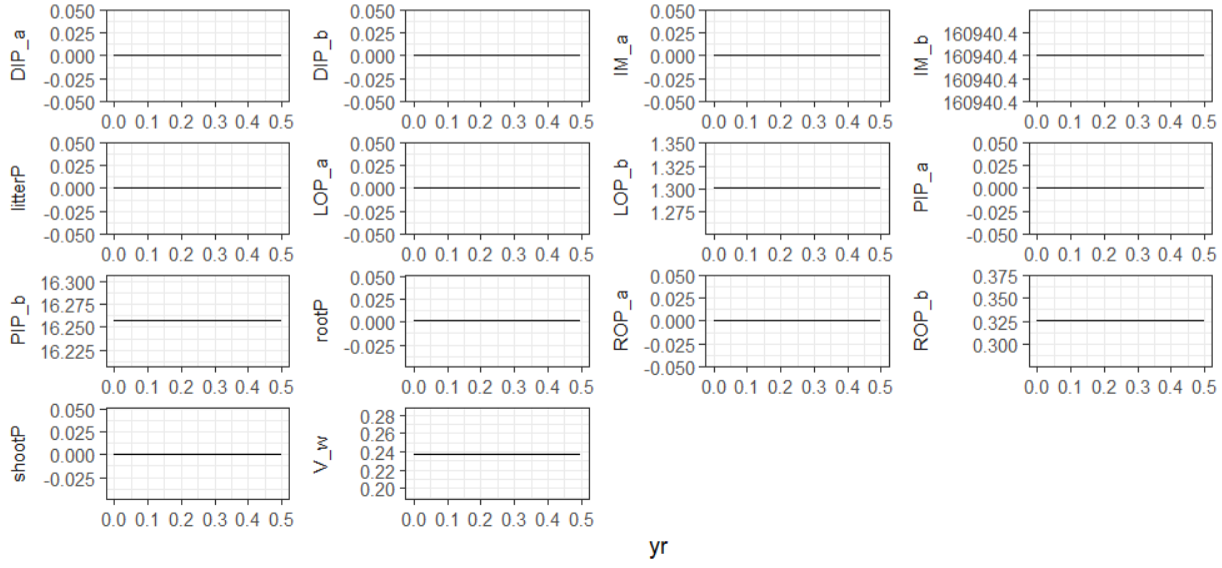
\includegraphics{C:/Users/Adrian.Wiegman/Documents/GitHub/wetlandP_2p1_stable/wetlandP_v2.1/documentation//fig1_states_W0_B0_G0.png}
\caption{1. all stocks should be constant through time}
\end{figure}

\hypertarget{dip-and-pip-should-equilibrate-no-other-stocks-should-change}{%
\paragraph{2. DIP and PIP should equilibrate, no other stocks should
change}\label{dip-and-pip-should-equilibrate-no-other-stocks-should-change}}

\begin{figure}
\centering
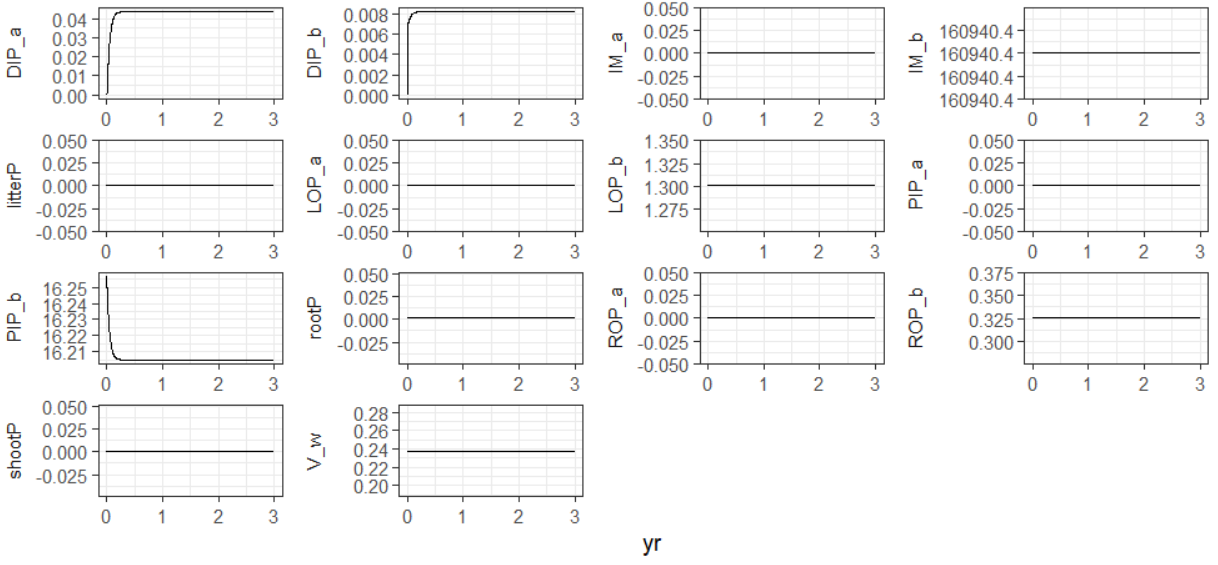
\includegraphics{C:/Users/Adrian.Wiegman/Documents/GitHub/wetlandP_2p1_stable/wetlandP_v2.1/documentation//fig2_states_W0_B0_G1.png}
\caption{2. DIP and PIP should equilibrate, no other stocks should
change}
\end{figure}

\hypertarget{shootp-rootp-lop-rop-should-fluctuuate-dip-and-pip-should-be-constant}{%
\paragraph{3. shootP, rootP, LOP, ROP should fluctuuate, DIP and PIP
should be
constant}\label{shootp-rootp-lop-rop-should-fluctuuate-dip-and-pip-should-be-constant}}

\begin{figure}
\centering
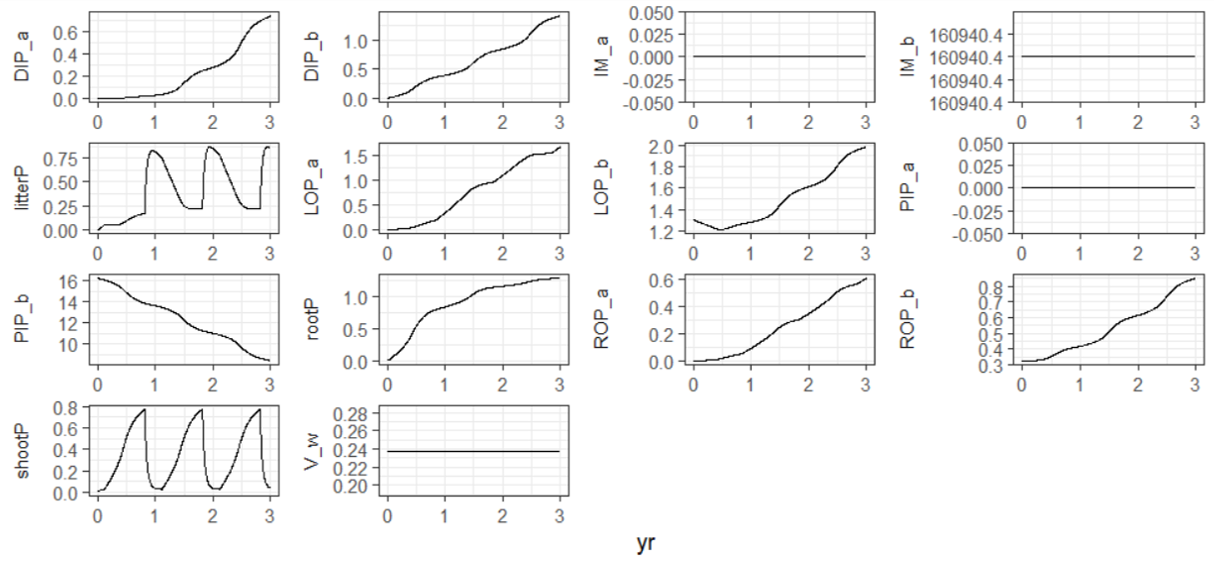
\includegraphics{C:/Users/Adrian.Wiegman/Documents/GitHub/wetlandP_2p1_stable/wetlandP_v2.1/documentation//fig3_states_W0_B1_G0.png}
\caption{3. shootP, rootP, LOP, ROP should fluctuuate, DIP and PIP
should be constant}
\end{figure}

\hypertarget{all-state-variables-should-fluctuate}{%
\paragraph{4. all state variables should
fluctuate}\label{all-state-variables-should-fluctuate}}

\begin{figure}
\centering
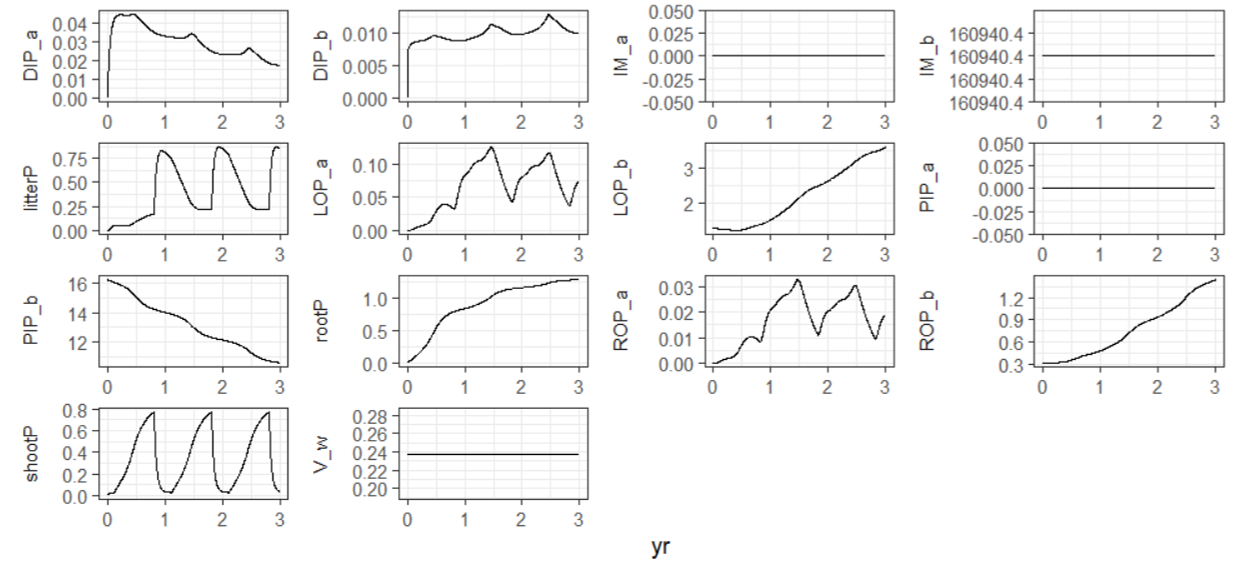
\includegraphics{C:/Users/Adrian.Wiegman/Documents/GitHub/wetlandP_2p1_stable/wetlandP_v2.1/documentation//fig4_states_W0_B1_G1.png}
\caption{4. all state variables should fluctuate}
\end{figure}

\hypertarget{volume-of-water-should-be-constant-through-time}{%
\paragraph{5. volume of water should be constant through
time}\label{volume-of-water-should-be-constant-through-time}}

\begin{figure}
\centering
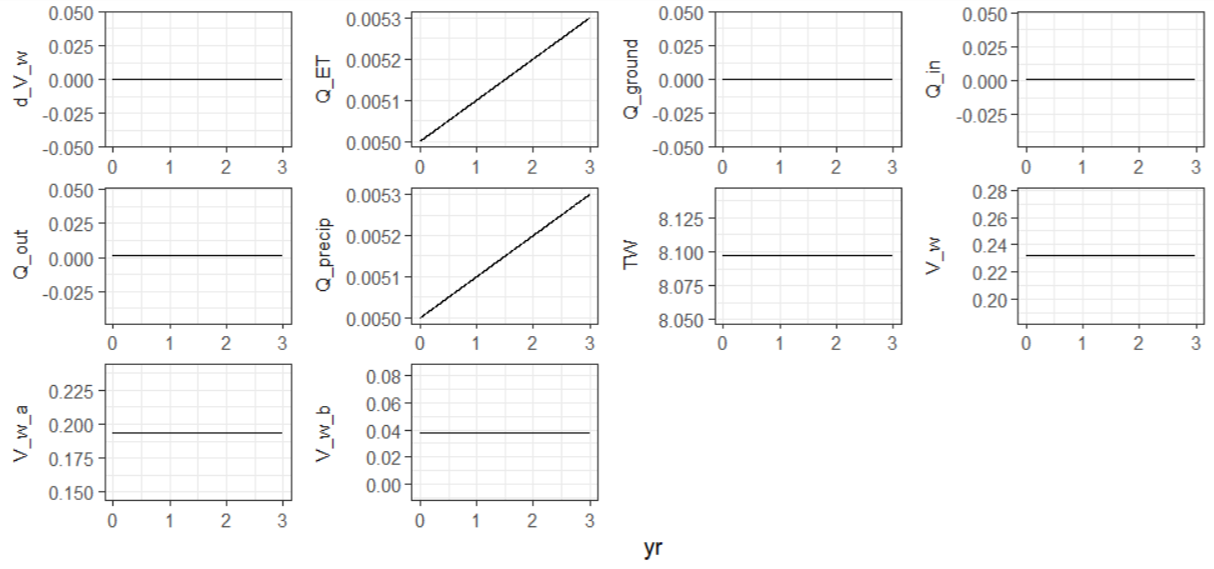
\includegraphics{C:/Users/Adrian.Wiegman/Documents/GitHub/wetlandP_2p1_stable/wetlandP_v2.1/documentation//fig5_hydroclimate_static_W1_B0_G0.png}
\caption{5. volume of water should be constant through time}
\end{figure}

\hypertarget{hydrocliamte-data-being-forced-on-the-model}{%
\paragraph{6. hydrocliamte data being forced on the
model}\label{hydrocliamte-data-being-forced-on-the-model}}

\begin{figure}
\centering
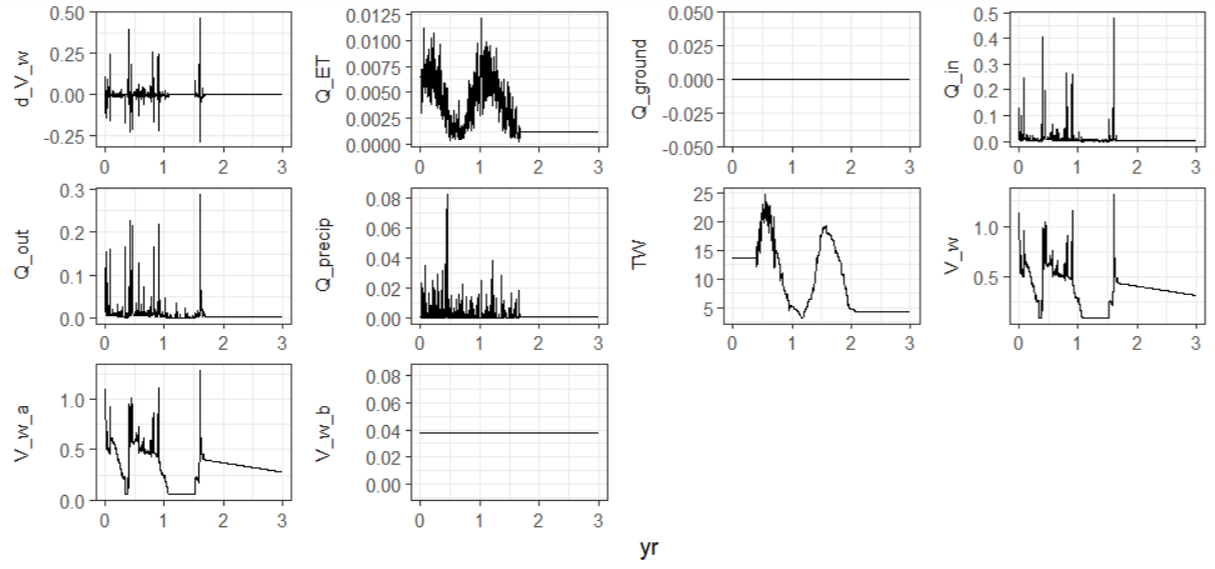
\includegraphics{C:/Users/Adrian.Wiegman/Documents/GitHub/wetlandP_2p1_stable/wetlandP_v2.1/documentation//fig6_hydroclimate_W1_B0_G0.png}
\caption{6. hydrocliamte data being forced on the model}
\end{figure}

\hypertarget{all-states-should-fluctuate-but-there-should-be-no-discontinuities-or-negative-values-inorganic-matter-compartment-should-be-constant-since-tss-0}{%
\paragraph{7. all states should fluctuate but there should be no
discontinuities, or negative values, inorganic matter compartment should
be constant since TSS =
0}\label{all-states-should-fluctuate-but-there-should-be-no-discontinuities-or-negative-values-inorganic-matter-compartment-should-be-constant-since-tss-0}}

\begin{figure}
\centering
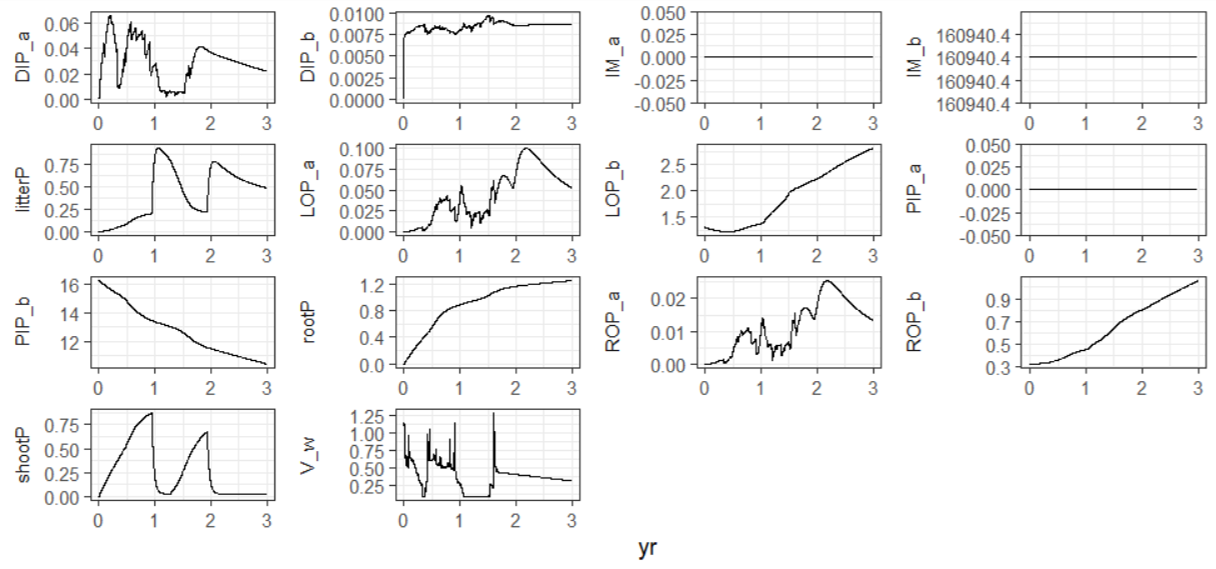
\includegraphics{C:/Users/Adrian.Wiegman/Documents/GitHub/wetlandP_2p1_stable/wetlandP_v2.1/documentation//fig7_states_W1_B1_G1.png}
\caption{7. all states should fluctuate but there should be no
discontinuities, or negative values, inorganic matter compartment should
be constant since TSS = 0}
\end{figure}

\hypertarget{concentrations-shoudl-fluctuate-but-have-no-sharp-discontinuities-or-negative-values}{%
\paragraph{8. concentrations shoudl fluctuate but have no sharp
discontinuities, or negative
values}\label{concentrations-shoudl-fluctuate-but-have-no-sharp-discontinuities-or-negative-values}}

\begin{figure}
\centering
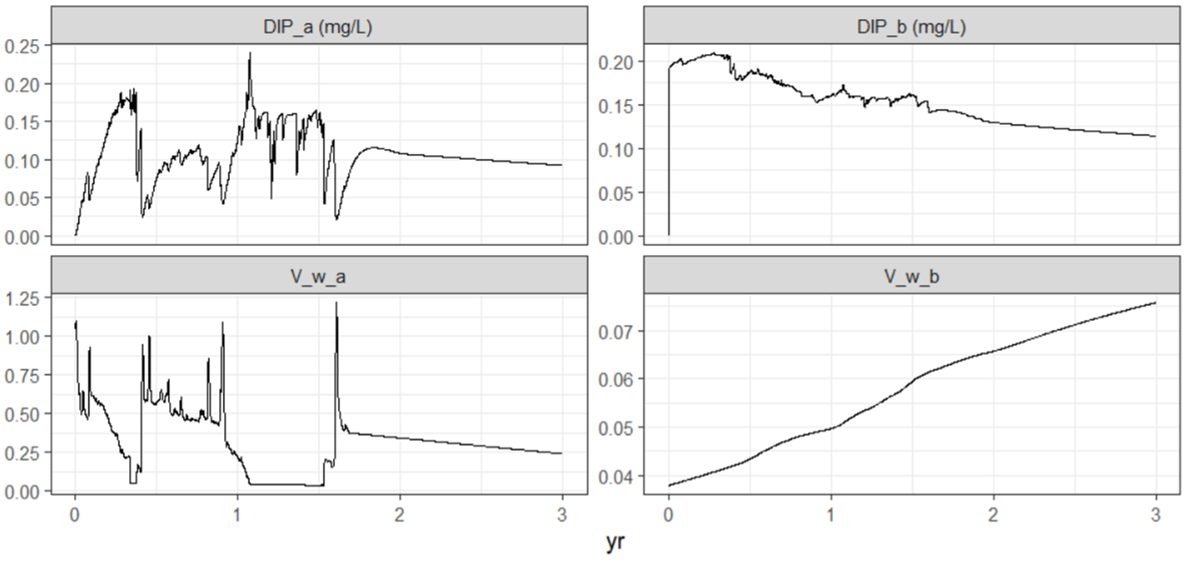
\includegraphics{C:/Users/Adrian.Wiegman/Documents/GitHub/wetlandP_2p1_stable/wetlandP_v2.1/documentation//fig8_DIP_A_W1_B1_G1.png}
\caption{8. concentrations shoudl fluctuate but have no sharp
discontinuities, or negative values}
\end{figure}

\hypertarget{references}{%
\subsection{References}\label{references}}

\hypertarget{online-data-sources}{%
\subsubsection{Online Data Sources}\label{online-data-sources}}

NOAA NCDC. National Oceanographic and Atmospheric Administration,
National Centers for Environmental Information, National Climatic Data
Center. United States Department of Commerce. URL: www.noaa.ncdc.gov
(accessed on 2021-10-25).

USGS NWIS. United States Geologic Survey, National Water Information
System. United States Department of the Interior. URL:
www.waterdata.usgs.gov (accessed on 2021-10-25).

VCGI. Vermont Open Geodata Portal, Vermont Center for Geographic
Information. AGENCY OF DIGITAL SERVICES. URL: www.geodata.vermont.gov
(acessed on 2021-10-25)

\hypertarget{scientific-literature}{%
\subsubsection{Scientific Literature}\label{scientific-literature}}

DeLaune, R. D., Baumann, R. H., \& Gosselink, J. G. (1983).
Relationships among Vertical Accretion, Coastal Submergence, and Erosion
in a Louisiana Gulf Coast Marsh. SEPM Journal of Sedimentary Research,
53(1), 147--157.
\url{https://doi.org/10.1306/212F8175-2B24-11D7-8648000102C1865D}

Hantush, M. M., Kalin, L., Isik, S., \& Yucekaya, A. (2013). Nutrient
Dynamics in Flooded Wetlands. I: Model Development. Journal of
Hydrologic Engineering, 18(12), 1709--1723.
\url{https://doi.org/10.1061/(ASCE)HE.1943-5584.0000741}

Marois, D. E., \& Mitsch, W. J. (2016). Modeling phosphorus retention at
low concentrations in Florida Everglades mesocosms. Ecological
Modelling, 319, 42-62.

Morris, J. T., Houghton, R. A., \& Botkin, D. B. (1984). Theoretical
limits of belowground production by Spartina alterniflora: An analysis
through modelling. Ecological Modelling, 26(3--4), 155--175.
\url{https://doi.org/10.1016/0304-3800(84)90068-1}

Morris, J. T., \& Bowden, W. B. (1986). A Mechanistic, Numerical Model
of Sedimentation, Mineralization, and Decomposition for Marsh
Sediments1. Soil Science Society of America Journal, 50(1), 96.
\url{https://doi.org/10.2136/sssaj1986.03615995005000010019x}

Morris, J. T., Sundareshwar, P. V., Nietch, C. T., Kjerfve, B., \&
Cahoon, D. R. (2002). Responses of coastal wetlands to rising sea level.
Ecology, 83(10), 2869-2877.

Morris, J. T., Barber, D. C., Callaway, J. C., Chambers, R., Hagen, S.
C., Hopkinson, C. S., \ldots{} Wigand, C. (2016). Contributions of
organic and inorganic matter to sediment volume and accretion in tidal
wetlands at steady state. Earth's Future, 4(4), 110--121.
\url{https://doi.org/de}

Reddy, K. R., \& Delaune, R. D. (2008). Biochemistry of wetland science
and application. CRC Press Taylor \& Francis Group, Boca Raton FL. ISBN
978-1-56670-678-0

Wang, N., \& Mitsch, W. J. (2000). A detailed ecosystem model of
phosphorus dynamics in created riparian wetlands. Ecological Modelling,
126(2--3), 101--130. \url{https://doi.org/10.1016/S0304-3800(00)00260-X}

Wang, H., Appan, A., \& Gulliver, J. S. (2003). Modeling of phosphorus
dynamics in aquatic sediments: I - Model development. Water Research.
\url{https://doi.org/10.1016/S0043-1354(03)00304-X}

Wiegman, A. R. H., Day, J. W., D'Elia, C. F., Rutherford, J. S., Morris,
J. T., Roy, E. D., \ldots{} Snyder, B. F. (2018). Modeling impacts of
sea-level rise, oil price, and management strategy on the costs of
sustaining Mississippi delta marshes with hydraulic dredging. Science of
the Total Environment, 618, 1547--1559.
\url{https://doi.org/10.1016/j.scitotenv.2017.09.314}

\hypertarget{software-dependancies}{%
\subsubsection{Software Dependancies}\label{software-dependancies}}

\$R

To cite R in publications use:

R Core Team (2023). R: A language and environment for statistical
computing. R Foundation for Statistical Computing, Vienna, Austria. URL
\url{https://www.R-project.org/}.

A BibTeX entry for LaTeX users is

@Manual\{, title = \{R: A Language and Environment for Statistical
Computing\}, author = \{\{R Core Team\}\}, organization = \{R Foundation
for Statistical Computing\}, address = \{Vienna, Austria\}, year =
\{2023\}, url = \{\url{https://www.R-project.org/}\}, \}

We have invested a lot of time and effort in creating R, please cite it
when using it for data analysis. See also `citation(``pkgname'')' for
citing R packages.

\$ggrepel

To cite package `ggrepel' in publications use:

Slowikowski K (2023). \emph{ggrepel: Automatically Position
Non-Overlapping Text Labels with `ggplot2'}. R package version 0.9.3,
\url{https://CRAN.R-project.org/package=ggrepel}.

A BibTeX entry for LaTeX users is

@Manual\{, title = \{ggrepel: Automatically Position Non-Overlapping
Text Labels with `ggplot2'\}, author = \{Kamil Slowikowski\}, year =
\{2023\}, note = \{R package version 0.9.3\}, url =
\{\url{https://CRAN.R-project.org/package=ggrepel}\}, \}

\$ecolMod

To cite package `ecolMod' in publications use:

Soetaert K, Herman PM (2022). \emph{ecolMod: ``A Practical Guide to
Ecological Modelling - Using R as a Simulation Platform''}. R package
version 1.2.6.4, \url{https://CRAN.R-project.org/package=ecolMod}.

A BibTeX entry for LaTeX users is

@Manual\{, title = \{ecolMod: ``A Practical Guide to Ecological
Modelling - Using R as a Simulation Platform''\}, author = \{Karline
Soetaert and Peter MJ Herman\}, year = \{2022\}, note = \{R package
version 1.2.6.4\}, url =
\{\url{https://CRAN.R-project.org/package=ecolMod}\}, \}

ATTENTION: This citation information has been auto-generated from the
package DESCRIPTION file and may need manual editing, see
`help(``citation'')'.

\$diagram

To cite package `diagram' in publications use:

Soetaert K (2020). \emph{diagram: Functions for Visualising Simple
Graphs (Networks), Plotting Flow Diagrams}. R package version 1.6.5,
\url{https://CRAN.R-project.org/package=diagram}.

A BibTeX entry for LaTeX users is

@Manual\{, title = \{diagram: Functions for Visualising Simple Graphs
(Networks), Plotting Flow Diagrams\}, author = \{Karline Soetaert\},
year = \{2020\}, note = \{R package version 1.6.5\}, url =
\{\url{https://CRAN.R-project.org/package=diagram}\}, \}

ATTENTION: This citation information has been auto-generated from the
package DESCRIPTION file and may need manual editing, see
`help(``citation'')'.

\$shape

To cite package `shape' in publications use:

Soetaert K (2021). \emph{shape: Functions for Plotting Graphical Shapes,
Colors}. R package version 1.4.6,
\url{https://CRAN.R-project.org/package=shape}.

A BibTeX entry for LaTeX users is

@Manual\{, title = \{shape: Functions for Plotting Graphical Shapes,
Colors\}, author = \{Karline Soetaert\}, year = \{2021\}, note = \{R
package version 1.4.6\}, url =
\{\url{https://CRAN.R-project.org/package=shape}\}, \}

ATTENTION: This citation information has been auto-generated from the
package DESCRIPTION file and may need manual editing, see
`help(``citation'')'.

\$rootSolve

To cite package `rootSolve' in publications use:

Soetaert K. and P.M.J. Herman (2009). A Practical Guide to Ecological
Modelling. Using R as a Simulation Platform. Springer, 372 pp.

Soetaert K. (2009). rootSolve: Nonlinear root finding, equilibrium and
steady-state analysis of ordinary differential equations. R-package
version 1.6

rootSolve was created to solve the examples from chapter 7 of our book -
please cite this book when using it, thank you! To see these entries in
BibTeX format, use `print(, bibtex=TRUE)', `toBibtex(.)', or set
`options(citation.bibtex.max=999)'.

\$rlang

To cite package `rlang' in publications use:

Henry L, Wickham H (2023). \emph{rlang: Functions for Base Types and
Core R and `Tidyverse' Features}. R package version 1.1.0,
\url{https://CRAN.R-project.org/package=rlang}.

A BibTeX entry for LaTeX users is

@Manual\{, title = \{rlang: Functions for Base Types and Core R and
`Tidyverse' Features\}, author = \{Lionel Henry and Hadley Wickham\},
year = \{2023\}, note = \{R package version 1.1.0\}, url =
\{\url{https://CRAN.R-project.org/package=rlang}\}, \}

\$Evapotranspiration

To cite package `Evapotranspiration' in publications use:

Guo D, Westra S, Peterson T (2022). \emph{Evapotranspiration: Modelling
Actual, Potential and Reference Crop Evapotranspiration}. R package
version 1.16,
\url{https://CRAN.R-project.org/package=Evapotranspiration}.

A BibTeX entry for LaTeX users is

@Manual\{, title = \{Evapotranspiration: Modelling Actual, Potential and
Reference Crop Evapotranspiration\}, author = \{Danlu Guo and Seth
Westra and Tim Peterson\}, year = \{2022\}, note = \{R package version
1.16\}, url =
\{\url{https://CRAN.R-project.org/package=Evapotranspiration}\}, \}

ATTENTION: This citation information has been auto-generated from the
package DESCRIPTION file and may need manual editing, see
`help(``citation'')'.

\$soiltexture

To cite package `soiltexture' in publications use:

Moeys J (2018). \emph{soiltexture: Functions for Soil Texture Plot,
Classification and Transformation}. R package version 1.5.1,
\url{https://CRAN.R-project.org/package=soiltexture}.

A BibTeX entry for LaTeX users is

@Manual\{, title = \{soiltexture: Functions for Soil Texture Plot,
Classification and Transformation\}, author = \{Julien Moeys\}, year =
\{2018\}, note = \{R package version 1.5.1\}, url =
\{\url{https://CRAN.R-project.org/package=soiltexture}\}, \}

\$zoo

To cite zoo in publications use:

Zeileis A, Grothendieck G (2005). ``zoo: S3 Infrastructure for Regular
and Irregular Time Series.'' \emph{Journal of Statistical Software},
\emph{14}(6), 1-27. \url{doi:10.18637/jss.v014.i06}
\url{https://doi.org/10.18637/jss.v014.i06}.

A BibTeX entry for LaTeX users is

@Article\{, title = \{zoo: S3 Infrastructure for Regular and Irregular
Time Series\}, author = \{Achim Zeileis and Gabor Grothendieck\},
journal = \{Journal of Statistical Software\}, year = \{2005\}, volume =
\{14\}, number = \{6\}, pages = \{1--27\}, doi =
\{10.18637/jss.v014.i06\}, \}

\$readxl

To cite package `readxl' in publications use:

Wickham H, Bryan J (2023). \emph{readxl: Read Excel Files}. R package
version 1.4.2, \url{https://CRAN.R-project.org/package=readxl}.

A BibTeX entry for LaTeX users is

@Manual\{, title = \{readxl: Read Excel Files\}, author = \{Hadley
Wickham and Jennifer Bryan\}, year = \{2023\}, note = \{R package
version 1.4.2\}, url =
\{\url{https://CRAN.R-project.org/package=readxl}\}, \}

\$diffeqr

To cite package `diffeqr' in publications use:

Rackauckas C, Nie Q (2017). ``DifferentialEquations.jl -- A Performant
and Feature-Rich Ecosystem for Solving Differential Equations in
Julia.'' \emph{The Journal of Open Source Software}, \emph{5}(1).
\url{doi:10.5334/jors.151} \url{https://doi.org/10.5334/jors.151}, R
package version 1.1.3,
\url{https://openresearchsoftware.metajnl.com/articles/10.5334/jors.151/}.

A BibTeX entry for LaTeX users is

@Article\{, doi = \{10.5334/jors.151\}, journal = \{The Journal of Open
Source Software\}, title = \{DifferentialEquations.jl -- A Performant
and Feature-Rich Ecosystem for Solving Differential Equations in
Julia\}, author = \{Chris Rackauckas and Qing Nie\}, year = \{2017\},
volume = \{5\}, number = \{1\}, url =
\{\url{https://openresearchsoftware.metajnl.com/articles/10.5334/jors.151/}\},
note = \{R package version 1.1.3\}, \}

\$deSolve

To cite package `deSolve' in publications use:

Karline Soetaert, Thomas Petzoldt, R. Woodrow Setzer (2010). Solving
Differential Equations in R: Package deSolve. Journal of Statistical
Software, 33(9), 1--25. \url{doi:10.18637/jss.v033.i09}

A BibTeX entry for LaTeX users is

@Article\{, title = \{Solving Differential Equations in \{R\}: Package
de\{S\}olve\}, author = \{\{Karline Soetaert\} and \{Thomas Petzoldt\}
and \{R. Woodrow Setzer\}\}, journal = \{Journal of Statistical
Software\}, volume = \{33\}, number = \{9\}, pages = \{1--25\}, year =
\{2010\}, doi = \{10.18637/jss.v033.i09\}, keywords = \{ordinary
differential equations, partial differential equations, differential
algebraic equations, initial value problems, R, FORTRAN, C\}, \}

\$lubridate

To cite lubridate in publications use:

Garrett Grolemund, Hadley Wickham (2011). Dates and Times Made Easy with
lubridate. Journal of Statistical Software, 40(3), 1-25. URL
\url{https://www.jstatsoft.org/v40/i03/}.

A BibTeX entry for LaTeX users is

@Article\{, title = \{Dates and Times Made Easy with \{lubridate\}\},
author = \{Garrett Grolemund and Hadley Wickham\}, journal = \{Journal
of Statistical Software\}, year = \{2011\}, volume = \{40\}, number =
\{3\}, pages = \{1--25\}, url =
\{\url{https://www.jstatsoft.org/v40/i03/}\}, \}

\$forcats

To cite package `forcats' in publications use:

Wickham H (2023). \emph{forcats: Tools for Working with Categorical
Variables (Factors)}. R package version 1.0.0,
\url{https://CRAN.R-project.org/package=forcats}.

A BibTeX entry for LaTeX users is

@Manual\{, title = \{forcats: Tools for Working with Categorical
Variables (Factors)\}, author = \{Hadley Wickham\}, year = \{2023\},
note = \{R package version 1.0.0\}, url =
\{\url{https://CRAN.R-project.org/package=forcats}\}, \}

\$stringr

To cite package `stringr' in publications use:

Wickham H (2022). \emph{stringr: Simple, Consistent Wrappers for Common
String Operations}. R package version 1.5.0,
\url{https://CRAN.R-project.org/package=stringr}.

A BibTeX entry for LaTeX users is

@Manual\{, title = \{stringr: Simple, Consistent Wrappers for Common
String Operations\}, author = \{Hadley Wickham\}, year = \{2022\}, note
= \{R package version 1.5.0\}, url =
\{\url{https://CRAN.R-project.org/package=stringr}\}, \}

\$dplyr

To cite package `dplyr' in publications use:

Wickham H, François R, Henry L, Müller K, Vaughan D (2023). \emph{dplyr:
A Grammar of Data Manipulation}. R package version 1.1.1,
\url{https://CRAN.R-project.org/package=dplyr}.

A BibTeX entry for LaTeX users is

@Manual\{, title = \{dplyr: A Grammar of Data Manipulation\}, author =
\{Hadley Wickham and Romain François and Lionel Henry and Kirill Müller
and Davis Vaughan\}, year = \{2023\}, note = \{R package version
1.1.1\}, url = \{\url{https://CRAN.R-project.org/package=dplyr}\}, \}

\$purrr

To cite package `purrr' in publications use:

Wickham H, Henry L (2023). \emph{purrr: Functional Programming Tools}. R
package version 1.0.1, \url{https://CRAN.R-project.org/package=purrr}.

A BibTeX entry for LaTeX users is

@Manual\{, title = \{purrr: Functional Programming Tools\}, author =
\{Hadley Wickham and Lionel Henry\}, year = \{2023\}, note = \{R package
version 1.0.1\}, url =
\{\url{https://CRAN.R-project.org/package=purrr}\}, \}

\$readr

To cite package `readr' in publications use:

Wickham H, Hester J, Bryan J (2023). \emph{readr: Read Rectangular Text
Data}. R package version 2.1.4,
\url{https://CRAN.R-project.org/package=readr}.

A BibTeX entry for LaTeX users is

@Manual\{, title = \{readr: Read Rectangular Text Data\}, author =
\{Hadley Wickham and Jim Hester and Jennifer Bryan\}, year = \{2023\},
note = \{R package version 2.1.4\}, url =
\{\url{https://CRAN.R-project.org/package=readr}\}, \}

\$tidyr

To cite package `tidyr' in publications use:

Wickham H, Vaughan D, Girlich M (2023). \emph{tidyr: Tidy Messy Data}. R
package version 1.3.0, \url{https://CRAN.R-project.org/package=tidyr}.

A BibTeX entry for LaTeX users is

@Manual\{, title = \{tidyr: Tidy Messy Data\}, author = \{Hadley Wickham
and Davis Vaughan and Maximilian Girlich\}, year = \{2023\}, note = \{R
package version 1.3.0\}, url =
\{\url{https://CRAN.R-project.org/package=tidyr}\}, \}

\$tibble

To cite package `tibble' in publications use:

Müller K, Wickham H (2023). \emph{tibble: Simple Data Frames}. R package
version 3.2.1, \url{https://CRAN.R-project.org/package=tibble}.

A BibTeX entry for LaTeX users is

@Manual\{, title = \{tibble: Simple Data Frames\}, author = \{Kirill
Müller and Hadley Wickham\}, year = \{2023\}, note = \{R package version
3.2.1\}, url = \{\url{https://CRAN.R-project.org/package=tibble}\}, \}

\$ggplot2

To cite ggplot2 in publications, please use

H. Wickham. ggplot2: Elegant Graphics for Data Analysis. Springer-Verlag
New York, 2016.

A BibTeX entry for LaTeX users is

@Book\{, author = \{Hadley Wickham\}, title = \{ggplot2: Elegant
Graphics for Data Analysis\}, publisher = \{Springer-Verlag New York\},
year = \{2016\}, isbn = \{978-3-319-24277-4\}, url =
\{\url{https://ggplot2.tidyverse.org}\}, \}

\$tidyverse

To cite package `tidyverse' in publications use:

Wickham H, Averick M, Bryan J, Chang W, McGowan LD, François R,
Grolemund G, Hayes A, Henry L, Hester J, Kuhn M, Pedersen TL, Miller E,
Bache SM, Müller K, Ooms J, Robinson D, Seidel DP, Spinu V, Takahashi K,
Vaughan D, Wilke C, Woo K, Yutani H (2019). ``Welcome to the
tidyverse.'' \emph{Journal of Open Source Software}, \emph{4}(43), 1686.
\url{doi:10.21105/joss.01686} \url{https://doi.org/10.21105/joss.01686}.

A BibTeX entry for LaTeX users is

@Article\{, title = \{Welcome to the \{tidyverse\}\}, author = \{Hadley
Wickham and Mara Averick and Jennifer Bryan and Winston Chang and Lucy
D'Agostino McGowan and Romain François and Garrett Grolemund and Alex
Hayes and Lionel Henry and Jim Hester and Max Kuhn and Thomas Lin
Pedersen and Evan Miller and Stephan Milton Bache and Kirill Müller and
Jeroen Ooms and David Robinson and Dana Paige Seidel and Vitalie Spinu
and Kohske Takahashi and Davis Vaughan and Claus Wilke and Kara Woo and
Hiroaki Yutani\}, year = \{2019\}, journal = \{Journal of Open Source
Software\}, volume = \{4\}, number = \{43\}, pages = \{1686\}, doi =
\{10.21105/joss.01686\}, \}

\$pacman

To cite pacman in publications, please use:

Rinker, T. W. \& Kurkiewicz, D. (2017). pacman: Package Management for
R. version 0.5.0. Buffalo, New York.
\url{http://github.com/trinker/pacman}

A BibTeX entry for LaTeX users is

@Manual\{, title = \{\{pacman\}: \{P\}ackage Management for \{R\}\},
author = \{Tyler W. Rinker and Dason Kurkiewicz\}, address = \{Buffalo,
New York\}, note = \{version 0.5.0\}, year = \{2018\}, url =
\{\url{http://github.com/trinker/pacman}\}, \}

\end{document}
